\documentclass[a4paper,pdflatex,11pt,mitminorthesis,singlespace,oneside]{cssethesis}
\renewcommand{\thesiscoursecode}{C6001}
%% Language and font encodings
\usepackage[english]{babel}
\usepackage[utf8x]{inputenc}
%%\usepackage[section]{placeins}
\usepackage{booktabs}
\usepackage{tabu}
\usepackage[T1]{fontenc}
\usepackage{enumitem}
\usepackage{pgf,tikz}
\usepackage{mathrsfs}
\usetikzlibrary{calc}
\usetikzlibrary{arrows}
%% Sets page size and margins

%% Useful packages
%% Code 
\usepackage{listings}
\usepackage{url}
\usepackage{subcaption}
\usepackage{graphicx}
\usepackage{float}
\usepackage{cite}

%%Algorithm
\usepackage{amsmath}
\usepackage[linesnumbered,ruled]{algorithm2e}

% list source code
\usepackage{listings}
% list style definition
\lstdefinestyle{customc}{language=C++,
  basicstyle=\footnotesize\ttfamily,
  numbers=left,
  stepnumber=1,
  showstringspaces=false,
  tabsize=1,
  breaklines=true,
  breakatwhitespace=false,
  backgroundcolor=\color{black!5}, % set backgroundcolor
}
\lstset{escapechar=@,style=customc}

%%Theorem
\usepackage{amsthm}
\theoremstyle{remark}
\newtheorem*{remark}{Remark}
\newtheorem{theorem}{Theorem}[section]
\newtheorem{property}{Property}[section]
\theoremstyle{definition}
\newtheorem{definition}{Definition}[section]
\newtheorem{claim}[theorem]{Claim}
\newtheorem{proposition}[theorem]{Proposition}
\newtheorem{lemma}[theorem]{Lemma}
\newtheorem{corollary}[theorem]{Corollary}
\newtheorem{conjecture}[theorem]{Conjecture}

\thesisauthor{Shizhe Zhao}
\thesisauthorlastname{Zhao}
\thesisdepartment{Caulfield School of Information Technology}
%                  Clayton School of Information Technology is the default
\thesisauthorstudentid{27505928} % Needed for litreview
\thesisauthoremail{szha414\@@student.monash.edu} % Optional. Note that the @ is
											 % given as \@@. This is not
											 % necessary in normal LaTeX,
											 % but it is if you use the
											 % amsmath package - so why not
											 % get into the habit?
%\thesismonth{July} % Optional. Current month is used if this is not set
%\thesisyear{2002} % Optional. Current year is used if this is not set
\thesistitle{Fast Obstacle Spatial Query Processing on Navigation Mesh}
\thesissupervisor{Assoc. Prof. David Taniar}

\begin{document}

\frontmatter					% start the thesis front matter.
\thesistitlepage				% Generate the title page.
\thesiscopyrightpage			% Generate the copyright page.
%\thesisdedicationpage			% Generate a dedication page (optional)
\tableofcontents				% Generate a table of contents.
%\listoftables					% Generate a list of tables (optional).
%\listoffigures					% Generate a list of figures (optional).
\pagebreak

\begin{thesisabstract}			% generate the abstract page.
Obstacle k-Nearest Neighbours problem is the k-Nearest Neighbour problem in a 
two-dimensional Euclidean plane with obstacles (\emph{OkNN}).
Existing and state of the art algorithms for OkNN are based on incremental 
visibility graphs and as such suffer from a well known disadvantage: costly 
and online visibility checking with quadratic worst-case running times.
In this research we develop a new OkNN algorithm which avoids these disadvantages
by representing the traversable space as a collection of convex polygons; i.e.
a Navigation Mesh. 
We then adapt a recent and optimal navigation mesh algorithm, \textit{Polyanya}, from the
single-source single-target setting to the the multi-target case. 
We also give two new and online heuristics for OkNN.
In a range of empirical comparisons, we show that our approach can be orders of magnitude faster than competing methods that rely on visibility graphs.
The work has been accepted for publication in \textit{Proceedings of the 11th Annual Symposium on Combinatorial Search (SoCS’2018), colocated with
IJCAI/ECAI’2018, July 2018 (Shizhe Zhao, David Taniar, Daniel Harabor, "Fast OkNN on Navigation
Mesh")}.

\textit{Keywords}: Obstacle Nearest Neighbor, kNN, Navigation Mesh, Spatial Search, Obstacle
Distance, Obstacle Navigation

\end{thesisabstract}                 

\chapter*{List of Publication}{
\begin{itemize}
\item \textit{Shizhe Zhao, David Taniar, Daniel Harabor, "Fast k-Nearest Neighbor On A Navigation
Mesh", Proceedings of the 11th Annual Symposium on Combinatorial Search (SoCS’2018), colocated with
IJCAI/ECAI’2018, July 2018}
\end{itemize}
\addcontentsline{toc}{chapter}{List of publications}
\pagebreak
}

\thesisdeclarationpage			% generate the declaration page (optional).

\begin{thesisacknowledgments}	% generate the acknowledgements page (optional).
I would like to thank my supervisors David Taniar and
  Daniel Harabor who bring me to the journey of this research.

\noindent
  I would like to thank my ICPC teammate Micheal Cui who present me the new work
  \textit{Polyanya}, which inspired me to propose new algorithms.

\end{thesisacknowledgments}  

%%%%%%%%%%%%%%%%%%%%%%%%%%%%%%%%%%%%%%%%%%%%%%%%%%%%%%%%%%%%%%%%%%%%%%%%%%%%%%
%%
%% Main matter 
%%
\mainmatter						% start the thesis body.

\chapter{Introduction}
\section{Overview}

Obstacle k-Nearest Neighbour (OkNN) is a common type of spatial analysis query 
which can be described as follows: given a set of target points and a 
collection of polygonal obstacles, all in two dimensions, find the $k$ 
closest targets to an a priori unknown query point $q$.
Such problems appear in a myriad of practical contexts.
For example, in an industrial warehouse setting a machine operator may be
interested to know the $k$ closest storage locations where a specific 
inventory item can be found. In competitive computer games meanwhile, agent 
AIs often rely on nearest-neighbour information to make strategic decisions 
such as during navigation, combat or resource gathering.

\begin{figure}[htp]
  \centering
  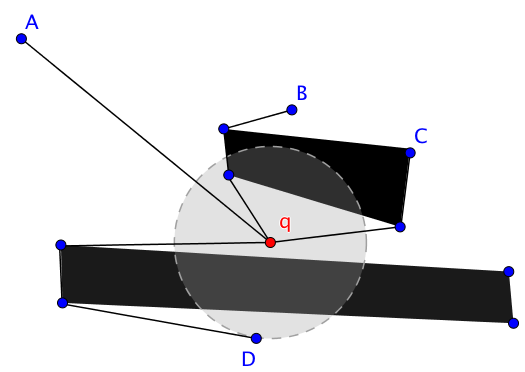
\includegraphics[width=\linewidth]{./pic/obs_dis.png}
  \caption{\small
  We aim to find the nearest neighbour of point $q$ from among the set of target points $A,B,C,D$. Black lines indicate the Euclidean shortest paths from $q$. Notice $D$ is the nearest neighbor of $q$ under the Euclidean metric but also the furthest neighbor of $q$ when obstacles are considered.}
\label{obs_dis}
\end{figure}

Traditional kNN queries in the plane (i.e. no obstacles) is a well studied
problem that can be handled by popular and well known algorithms including
~\textit{KD-Tree}~\cite{ooi1987spatial} and
\textit{R-tree}~\cite{guttman1984r}.  
%and other successful /variants\cite{beckmann1990r,sellis1987r+,kamel1993hilbert}).  
These methods organise the collection of target points into a hierarchical structure 
that serves to: (i) quickly identify a set of nearest neighbour candidates and; (ii) helps 
prune those candidates to return the $k$ closest.  A key ingredient to the success of
these algorithms is the Euclidean metric which provides perfect
distance information between any pair of points.  When obstacles are
introduced however the Euclidean metric becomes an often misleading
lower-bound. Figure~\ref{obs_dis} shows such an example.

Two popular algorithms for OkNN, which can deal with obstacles, are
\emph{local visibility graphs}~\cite{zhang2004spatial} and \emph{fast
filter}~\cite{xia2004fast}. Though different in details, both of these methods
are similar in that they depend on the incremental and online construction of 
a graph of co-visible points. Algorithms of this type are simple to understand, 
provide optimality guarantees and the promise of fast performance. 
Such advantages make incremental visibility graphs attractive to researchers 
and, despite more than a decade since their introduction, they continue to 
appear as ingredients in a variety of kNN studies from the literature; e.g. 
~\cite{gao2011efficient,gao2016reverse,gao2009continuous}.
However, incremental visibility graphs also suffer from a number of notable 
disadvantages including:
(i) online visibility checks;
(ii) an incremental construction process that has up to quadratic space and 
time complexity for the worst case;
(iii) duplicated effort, since the graph is discarded each time the query 
point changes.

In this paper we develop a new method for computing kNN in the presence of
obstacles which avoids these same disadvantages.  Our work extends
Polyanya~\cite{cuicompromise}: a recent and very fast algorithm for computing
Euclidean shortest paths on a navigation mesh: a data structure comprised of
convex polygons which taken together represent the entire traversable space.  
Compared to visibility graphs, navigation meshes are much cheaper to construct and
sometimes available as input ``for free'' (e.g. in computer game settings, navigation
meshes are often created, at least in part, by human designers).  
We describe how Polyanya can be generalised, from point-to-point problems to the
multi-target case. We also develop along the way two new, efficient and online heuristics
which can be used for OkNN.  Finally, we compare our work against incremental
visibility graphs in a wide range of experimental settings where we show that
Polyanya is in some cases three orders of magnitude faster.

The rest of the paper is organised as follows: (i) we give a description of the Obstacle kNN 
problem and associated technical terms; (ii) we review key components of
Polyanya; (iii) we give a formal description of our proposed algorithms including proofs and pseudocode;
(iv) experimental results and discussion and; (v) concluding thoughts.


\chapter{Literature Review}\label{lreview}
\section{Overview}\label{lroverview}
As we've mentioned in previous chapter, OkNN problem appears in both
AI path planning and Spatial query processing. Therefore, this literature review includes
related works in these two fields.

In section~\ref{lrai}, we introduce two classic pathfinding algorithms:
\textit{Dijkstra} and \textit{A*}, as the historic background.
In section~\ref{lrindex}, we introduce a spatial index \textit{R-tree},
and discuss how it solves traditional kNN problem.
In section~\ref{lrknn}, we focus on existing works on OkNN, two algorithms based on
\textit{Local Visibility Graph} will be discussed. 
In section~\ref{lrnav}, we introduce a very fast point-to-point algorithm in AI path planning
field which shows a new direction to solve OkNN problem.
In section~\ref{lrquery}, we briefly discuss other related spatial queries which can be
improved by our research.

\section{Classic pathfinding}\label{lrai}
The most widely used pathfinding algorithm is \textit{Dijkstra} \cite{dijkstra1959note}. 
The algorithm works on a nonnegative weighted graph, it requires a priority queue and
regards the length of shortest path as key, and it visit vertices in the order
of lenght of shortest path until requirements be satisfied, e.g. the target has been found.
When the target is the furthest vertex to the start vertex, \textit{Dijkstra} has to explore the entire
map. Based on such consideration, researchers generalized \textit{Dijkstra} algorithm to
\textit{best-first search} which explores a graph by expanding the most promising node chosen
acording to a specified rule.
\textit{A*} \cite{hart1968formal} is known as a famous \textit{best-first search},
it select the path that minimizes:
$$
f(n) = \textit{g-value}(n) + \textit{h-value}(n)
$$
where $n$ is the last node on the path, \textit{g-value} is the length of shortest path from start to
$n$, \textit{h-value} is a estimation of shortest path from $n$ to the goal which is
problem-specific. One important propert of \textit{h-value} is admissibility, meaning that it never
overestimates the actual cost to the target.
For example, in an Euclidean plane with obstacles, \textit{h-value} can be the Euclidean
distance.

In following sections and the chapter~\ref{proposedalgo}, we will show how \textit{Dijkstra} and
\textit{A*} algorithms be applied on the OkNN problem.

\section{Spatial Index}\label{lrindex}

\subsection{\textit{R-tree}}

\textit{R-tree} has many variations\cite{guttman1984r,beckmann1990r,sellis1987r+,kamel1993hilbert},
they improve efficiency in different aspects,
but they still provide same functionality,
so we only introduce the classic \textit{R-tree} in this section.

\begin{figure}[htp]
  \centering
  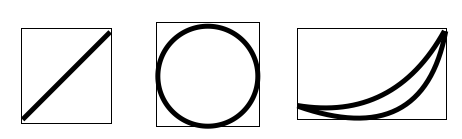
\includegraphics[width=.8\linewidth]{pic/mbr.PNG}
  \caption{\small Both segments, circle and irregular shape can be represented by their MBR}
  \label{mbr}
\end{figure}

\textit{R-tree} is a heighb-balanced tree \cite{guttman1984r}, all objects are stored in leaf
node. In leaf node, if an object is not a point, it would be represented by its \textit{Minimal Bounding
Rectangle} (MBR), figure~\ref{mbr} shows example of MBRs. Each interior node is also
represented by a MBR which contains either leaf nodes or descendant interior nodes.
To guarantee efficiency, each non-root node of \textit{R-tree} can contain at least $m$ entries
and at most $M$ entries, where $m, M$ are specified constant when \textit{R-tree} is built, and
\textit{R-tree}'s root alway has two entries. 
Usually, objects retrieval start from the root,
then narrow down to children nodes based on spatial information in their MBRs, and finally
retrieve objects from leaf nodes.
Figure~\ref{rtree} shows how to store and retrieve objects.

\begin{figure}[htp]
  \centering
  \begin{subfigure}{.5\textwidth}
    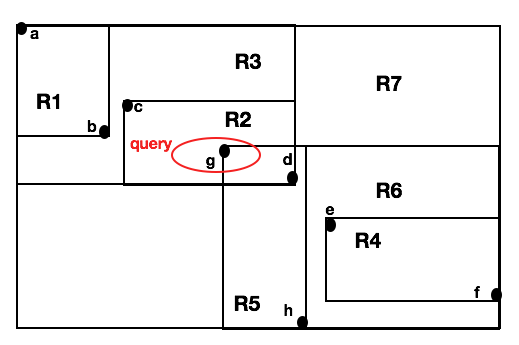
\includegraphics[width=\linewidth]{pic/hierarchy_mbr.PNG}
    \caption{Hierachy of MBRs}
    \label{hmbr}
  \end{subfigure}%
  \begin{subfigure}{.5\textwidth}
    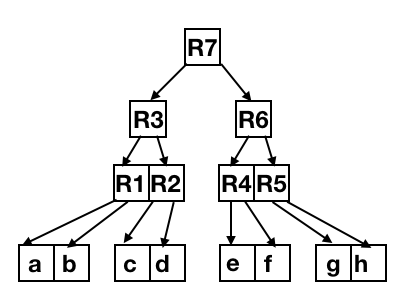
\includegraphics[width=\linewidth]{pic/rtree.PNG}
    \caption{Corresponding tree structure}
    \label{tree}
  \end{subfigure}
  \caption{\small $\{a,b,c,d,e,f,g,h\}$ is the object set,
  $R1,R2,R4,R5$ are leaf nodes, $R3,R6$ are interior nodes, and $R7$ is the root.
  The red oval is a range query, starting with $R7$, since $R6$'s MBR overlapped with query
  area, we narrow down to $R6$, then to $R5$, and finally retrieve $g$. Notice that $R3,R2$ also
  overlap with the query, so they will also be visited, but nothing retrieved.
  }
  \label{rtree}
\end{figure}

From the example in figure~\ref{rtree}, we can see that overlapping area will be explored
multiplel times in retrieval progress, which duplicated efforts.
Thus, some variants use strict non-overlapping interior node (e.g.
$R^+\textit{-tree}$\cite{sellis1987r+}), and non-overlapping \textit{R-tree} is a wide topic in
spatial index which beyond the scope of this thesis.

\subsection{Nearest Neighbor Query}
In the \textit{R-tree}, all nodes are organized by their spatial information,
so that the nearest neighbor of a point can be retrieved by exploring tree nodes in some order.
To introduce the algorithm, we need to discuss two metrics: given query point $q$ and the MBR of a tree node
\begin{itemize}
  \item \textit{\textbf{mindist}} is the minimal distance from $q$ to the MBR, it estimates the
    distance from $q$ to inside object, so this metric is the priority of the tree node;
  \item \textit{\textbf{minmaxdist}} is the uppber bound of the NN distance of any object inside
    the MBR, if the $mindist$ of any MBR large than this value, then such MBR cannot contains
    the nearest object, so this metric is for pruning.
\end{itemize}
The algorithm starts with root node and proceeds down the tree. When it visits a leaf node,
current nearest neighbor will be updated;
When it visits a non-leaf node, the children of such node is sorted by \textit{mindist}, and pruned by
\textit{minmaxdist}, then algorithm does \textit{depth-first-search} on ordered and pruned children nodes;
when algorithm finished, the updated nearest neighbor is the answer, and it can be easily
generalized to finding kNN by changes below:
\begin{itemize}
  \item  Tracking k current nearest neighbors, instead of one.
  \item  The pruning is according to the current k-th nearest neighbor.
\end{itemize}

This kind of algorithm is called \textit{branch-and-bound} traversal, which has been well
studied and widely used in other artifical intelligence areas\cite{sellis1987r+},
and existing NN queries are based on it with different ordering and pruning strategies,
more details are in \cite{roussopoulos1995nearest,cheung1998enhanced}.

\section{Obstacle k-Nearest Neighbor}\label{lrknn}

In OkNN problem, the metric is obstacle distance,
so all existing OkNN algorithms are actually Obstacle Distance Computation (ODC).
In following subsections, we introduce these ODC algorithms and show how to apply them on OkNN.

\subsection{In-main-memory OkNN}
Solving obstacle path problems in-main-memory has been well studied \cite{de2000computational},
these works need to compute visibility graph which any pair of co-visible vertices has en edge,
figure~\ref{vg} shows an example.
\begin{figure}[htp]
  \centering
  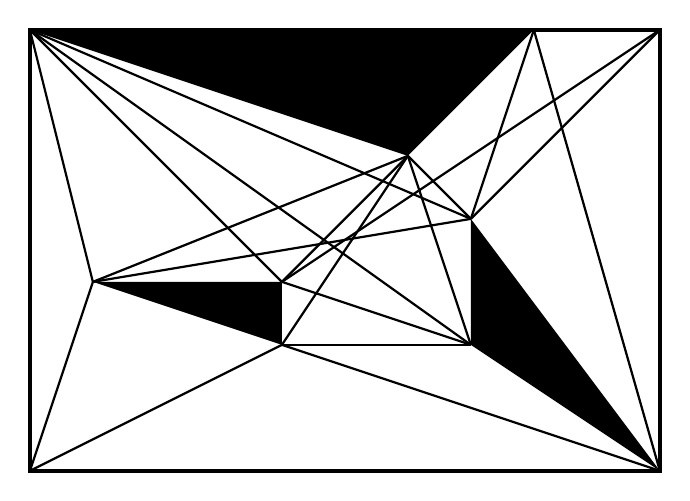
\begin{tikzpicture}[scale=0.8]
  %\includegraphics[width=.6\linewidth]{pic/vg.png}
    %\coordinate (a) at (2, 6); 
\coordinate (a) at (0, 7);
\coordinate (b) at (8, 7); 
\coordinate (c) at (6, 5); 
\coordinate (d) at (1, 3);
\coordinate (e) at (4, 3);
\coordinate (f) at (4, 2);
\coordinate (g) at (7, 4);
\coordinate (h) at (7, 2);
%\coordinate (i) at (9, 0);
\coordinate (i) at (10, 0);
\coordinate (j) at (5, 2);
\coordinate (k) at (0, 7);
\coordinate (l) at (0, 0);
\coordinate (m) at (10, 0);
\coordinate (n) at (10, 7);
\coordinate (q) at (3, 4);
\coordinate (Q) at (3, 4);
\coordinate (t) at (9, 3);
\coordinate (o) at (7.5, 5.5);

\newcommand{\nodelabel}[2] {
    \node[fill,circle,scale=0.25,label=#2:$#1$,color=red] at (#1) {$#1$};
}

\newcommand{\medge}[2]{
    \draw[gray,thick] (#1)--(#2);
}

\newcommand{\vgedge}[2]{
    \draw[black,thick] (#1)--(#2);
}

\newcommand{\drawVs}{
    %\nodelabel{a}{above}
    \nodelabel{b}{below}
    \nodelabel{c}{below}
    
    %\nodelabel{d}{left}
    \nodelabel{e}{right}
    \nodelabel{f}{below}
    
    \nodelabel{g}{above}
    \nodelabel{h}{below}
    %\nodelabel{i}{below}
}

\newcommand{\drawmeshs}{
    \medge{a}{k},\medge{a}{d},\medge{a}{b},\medge{a}{c}
    \medge{b}{c},
    \medge{c}{g}
    \medge{d}{f},\medge{d}{l},\medge{d}{e}
    \medge{l}{f}
    \medge{e}{c},\medge{e}{f}
    \medge{f}{h}
    \medge{g}{h},\medge{g}{b}
    \medge{h}{i}
}

\newcommand{\drawobstacles}{
    \fill[black] (a)--(b)--(c)--cycle;
    \fill[black] (g)--(h)--(i)--cycle;
    \fill[black] (d)--(e)--(f)--cycle;
}

\newcommand{\drawstart} {
    % \fill[blue] (q) circle[radius=.5ex];
    % \node[above] at (q) {$q$};
    \node[fill,circle,scale=0.25,label=above:$q$,color=blue] at (q) {$q$};

}

\newcommand{\drawend}{
    \fill[blue] (t) circle[radius=.5ex];
    \node[above] at (t) {$t$};
}

\newcommand{\drawboundary}{
    \draw[black, ultra thick] (k)--(n)--(m)--(l)--cycle;
}

\newcommand{\showvisible} {
    \fill[lightgray] (c)--(e)--(d)--(a);
    \nodelabel{e}{right}
    \nodelabel{c}{below}
    \drawstart;
}

\newcommand{\stepa} {
    \fill[lightgray] (c)--(e)--(d)--(a);
    \fill[lightgray] (c)--(g)--(h)--(f)--(e);
    \draw[black, thin] (q)--(g);
    \draw[green, very thick] (e)--(c);
    \drawstart
    \drawVs
}

\newcommand{\stepb} {
    \fill[lightgray] (c)--(e)--(d)--(a);
    \fill[lightgray] (c)--(g)--(h)--(f)--(e);
    \fill[lightgray] (c)--(g)--(b);
    \draw[black, thin] (q)--(g);
    \draw[green, very thick] (e)--(c);
    \draw[black, thin] (g)--(t);
    \draw[black, thin] (q)--(g);
    \draw[green, very thick] (g)--(c);
    \draw[green, very thick] (g)--(b);
    \drawstart
    \drawend
    \drawVs
}

\newcommand{\polyanyaexpand}{
    \draw[black,very thin, dashed] (q)--($(q)!5cm!(e)$);
    \draw[black,very thin, dashed] (q)--($(q)!5cm!(c)$);
    \draw[orange!50, line width=3pt] (j)--(h);
    \draw[orange!50, line width=3pt] (h)--(g);
    \draw[orange!50, line width=3pt] (g)--(c);
    \draw[cyan, line width=3pt] (e)--(f);
    \draw[cyan, line width=3pt] (f)--(j);
}

\newcommand{\drawVG}{
    \vgedge{a}{d},\vgedge{a}{e},\vgedge{a}{g},\vgedge{a}{h}
    \vgedge{b}{g},\vgedge{b}{m}
    \vgedge{c}{d},\vgedge{c}{e},\vgedge{c}{g},\vgedge{c}{f},\vgedge{c}{h}
    \vgedge{d}{l},\vgedge{d}{g}
    \vgedge{e}{h},\vgedge{e}{n}
    \vgedge{f}{l},\vgedge{f}{h},\vgedge{f}{m}
    \vgedge{g}{n}
}
\newcommand{\drawmap}{
    \drawboundary
    \drawobstacles
    \drawmeshs
    \drawVs
    \drawstart
    \drawend
}

\newcommand{\intervalexpansion}{
    \drawboundary
    \drawobstacles
    \drawmeshs
    {\draw[green!50, line width=3pt, dashed] (e)--(d);}
    {\draw[green!50, line width=3pt, dashed] (d)--(a);}
    {\draw[green!50, line width=3pt, dashed] (a)--(c);}
    {\draw[green!50, line width=3pt, dashed] (e)--(c);}
    {\draw[green!50, line width=3pt, dashed] (d)--(l);}
    {\draw[green!50, line width=3pt, dashed] (e)--(f);}
    {\draw[green!50, line width=3pt, dashed] (f)--(j);}
    {\draw[green!50, line width=3pt, dashed] (j)--(h);}
    {\draw[green!50, line width=3pt, dashed] (g)--(h);}
    {\draw[green!50, line width=3pt, dashed] (c)--(g);}
    {\draw[green!50, line width=3pt, dashed] (g)--(b);}
    {\draw[black, line width=3pt] (q)--(g);}
    {\draw[black, line width=3pt] (g)--(t);}
    \drawstart
    \drawend 
    \drawVs
}

    \drawboundary
    \drawobstacles
    \drawVG
  \end{tikzpicture}
  \caption{\small The rectangle is the boundary of the map, black polyogns are obstacles, and all
  black lines are edge in the visibility graph.}
  \label{vg}
\end{figure}

Since all edges of the shortest path belong to visibility graph \cite{lozano1979algorithm},
once precomputed it and include visible edges from query point, we can run shortest path
algorithm (e.g. \textit{Dijkstra}) to find k-nearest neighbor.
However, precomputing visibility graph(VG) is costly:
even the best algorithm \cite{ghosh1991output} has
$O(m + nlogn)$ runtime, where $n$ is the number of vertex and $m$ is the number edges,
and in practice $m$ can reach to $O(n^2)$.
In spatial database scenario, $n$ can be more than $10,000$, so in-main-memory approach is not
suitable for spatial database scenario.

\subsection{Local Visibility Graph}

Since building global VG is infeasible, researchers in spatial database field
are motivated to design an algorithm that only consider query related area.

In 2004, Zhang proposed the \textit{Local Visibility Graph} (LVG) algorithm\cite{zhang2004spatial}
to compute obstacle distance.
Assume obstacles are stored in \textit{R-tree},
given query point $q$, and a target $t$, the algorithm runs in
following way:
\begin{enumerate}
    \item It starts with a small VG centered on $q$ with radius $r=d_e(q, t)$ (figure~\ref{edbt1});
    \item Then compute shortest path on current VG (figure~\ref{edbt2});
    \item Enlarge the circle to current obstacle distance $r=d_o(q,t)$, update the VG
      incrementally (figure~\ref{edbt2}) and recompute the shortest path (figure~\ref{edbt4});
    \item Repeat the previous step until $r>=d_o(q, t)$.
\end{enumerate}

\begin{figure*}[!h]
  \begin{subfigure}{\linewidth}
    \centering
    \begin{subfigure}{.45\linewidth}
      \centering
      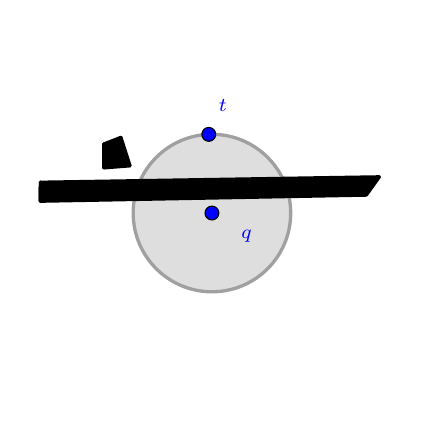
\begin{tikzpicture}[line cap=round,line join=round,>=triangle 45,x=1.0cm,y=1.0cm]
\definecolor{aqaqaq}{rgb}{0.6274509803921569,0.6274509803921569,0.6274509803921569}
\definecolor{qqqqff}{rgb}{0.,0.,1.}
\clip(1.6,0.47) rectangle (6.28,5.17);
\draw [line width=1.2pt,color=aqaqaq,fill=aqaqaq,fill opacity=0.3499999940395355] (3.9400050555577426,2.815716717828029) circle (1.cm);
\fill[line width=1.2pt,fill=black,fill opacity=1.0] (1.7619906352802,3.2064019550048823) -- (1.760948257574785,2.966272798087264) -- (5.9009925693289444,3.0440732742639014) -- (6.065992717197827,3.275305213897039) -- cycle;
\fill[line width=1.2pt,fill=black,fill opacity=1.0] (2.7838752248591803,3.776985670170509) -- (2.5711486339617498,3.69319853872332) -- (2.5711499019374466,3.389901746844879) -- (2.8995061535758593,3.4158740479215886) -- cycle;
\draw [line width=1.2pt] (1.7619906352802,3.2064019550048823)-- (1.760948257574785,2.966272798087264);
\draw [line width=1.2pt] (1.760948257574785,2.966272798087264)-- (5.9009925693289444,3.0440732742639014);
\draw [line width=1.2pt] (5.9009925693289444,3.0440732742639014)-- (6.065992717197827,3.275305213897039);
\draw [line width=1.2pt] (6.065992717197827,3.275305213897039)-- (1.7619906352802,3.2064019550048823);
\draw [line width=1.2pt] (2.7838752248591803,3.776985670170509)-- (2.5711486339617498,3.69319853872332);
\draw [line width=1.2pt] (2.5711486339617498,3.69319853872332)-- (2.5711499019374466,3.389901746844879);
\draw [line width=1.2pt] (2.5711499019374466,3.389901746844879)-- (2.8995061535758593,3.4158740479215886);
\draw [line width=1.2pt] (2.8995061535758593,3.4158740479215886)-- (2.7838752248591803,3.776985670170509);
\draw [line width=1.2pt] (1.760948257574785,2.9662727980872643)-- (1.7619906352802033,3.206401955004883);
\begin{scriptsize}
\draw [fill=qqqqff] (3.9400050555577426,2.815716717828029) circle (2.5pt);
\draw[color=qqqqff] (4.380260269409033,2.521369672358508) node {$q$};
\draw [fill=qqqqff] (3.8997931043534932,3.8149078902171505) circle (2.5pt);
\draw[color=qqqqff] (4.079705546011023,4.182329985873814) node {$t$};
\end{scriptsize}
\end{tikzpicture}
      \caption{
        \small 
        the long rectangle obstacle in the\\
        circle is retrieved and included in vg.
      }
      \label{edbt1}
    \end{subfigure}%
    \begin{subfigure}{.45\linewidth}
      \centering
      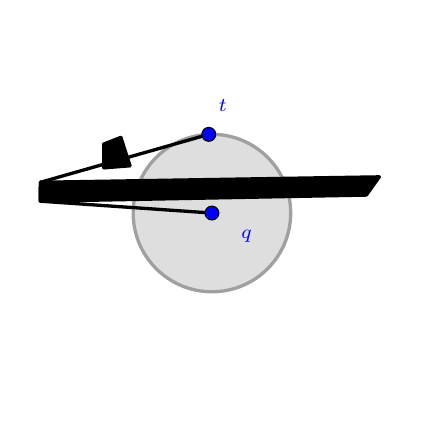
\begin{tikzpicture}[line cap=round,line join=round,>=triangle 45,x=1.0cm,y=1.0cm]
\definecolor{aqaqaq}{rgb}{0.6274509803921569,0.6274509803921569,0.6274509803921569}
\definecolor{qqqqff}{rgb}{0.,0.,1.}
\clip(1.6,0.47) rectangle (6.28,5.17);
\draw [line width=1.2pt,color=aqaqaq,fill=aqaqaq,fill opacity=0.3499999940395355] (3.9400050555577426,2.815716717828029) circle (1.cm);
\fill[line width=1.2pt,fill=black,fill opacity=1.0] (1.7619906352802,3.2064019550048823) -- (1.760948257574785,2.966272798087264) -- (5.9009925693289444,3.0440732742639014) -- (6.065992717197827,3.275305213897039) -- cycle;
\fill[line width=1.2pt,fill=black,fill opacity=1.0] (2.7838752248591803,3.776985670170509) -- (2.5711486339617498,3.69319853872332) -- (2.5711499019374466,3.389901746844879) -- (2.8995061535758593,3.4158740479215886) -- cycle;
\draw [line width=1.2pt] (1.7619906352802,3.2064019550048823)-- (1.760948257574785,2.966272798087264);
\draw [line width=1.2pt] (1.760948257574785,2.966272798087264)-- (5.9009925693289444,3.0440732742639014);
\draw [line width=1.2pt] (5.9009925693289444,3.0440732742639014)-- (6.065992717197827,3.275305213897039);
\draw [line width=1.2pt] (6.065992717197827,3.275305213897039)-- (1.7619906352802,3.2064019550048823);
\draw [line width=1.2pt] (2.7838752248591803,3.776985670170509)-- (2.5711486339617498,3.69319853872332);
\draw [line width=1.2pt] (2.5711486339617498,3.69319853872332)-- (2.5711499019374466,3.389901746844879);
\draw [line width=1.2pt] (2.5711499019374466,3.389901746844879)-- (2.8995061535758593,3.4158740479215886);
\draw [line width=1.2pt] (2.8995061535758593,3.4158740479215886)-- (2.7838752248591803,3.776985670170509);
\draw [line width=1.2pt] (3.9400050555577426,2.815716717828029)-- (1.760948257574785,2.9662727980872643);
\draw [line width=1.2pt] (1.760948257574785,2.9662727980872643)-- (1.7619906352802033,3.206401955004883);
\draw [line width=1.2pt] (1.7619906352802033,3.206401955004883)-- (3.8997931043534932,3.8149078902171505);
\begin{scriptsize}
\draw [fill=qqqqff] (3.9400050555577426,2.815716717828029) circle (2.5pt);
\draw[color=qqqqff] (4.380260269409033,2.521369672358508) node {$q$};
\draw [fill=qqqqff] (3.8997931043534932,3.8149078902171505) circle (2.5pt);
\draw[color=qqqqff] (4.079705546011023,4.182329985873814) node {$t$};
\end{scriptsize}
\end{tikzpicture}
      \caption{
        \small current shortest path may be blocked by some obstacles outside
      }
      \label{edbt2}
    \end{subfigure}
  \end{subfigure}\par\medskip
  \begin{subfigure}{\linewidth}
    \centering
    \begin{subfigure}{.45\linewidth}
      \centering
      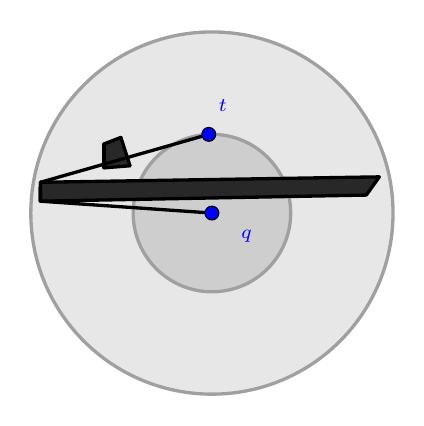
\begin{tikzpicture}[line cap=round,line join=round,>=triangle 45,x=1.0cm,y=1.0cm]
\definecolor{aqaqaq}{rgb}{0.6274509803921569,0.6274509803921569,0.6274509803921569}
\definecolor{qqqqff}{rgb}{0.,0.,1.}
\clip(1.6,0.47) rectangle (6.28,5.17);
\draw [line width=1.2pt,color=aqaqaq,fill=aqaqaq,fill opacity=0.3499999940395355] (3.9400050555577426,2.815716717828029) circle (1.cm);
\fill[line width=1.2pt,fill=black,fill opacity=1.0] (1.7619906352802,3.2064019550048823) -- (1.760948257574785,2.966272798087264) -- (5.9009925693289444,3.0440732742639014) -- (6.065992717197827,3.275305213897039) -- cycle;
\fill[line width=1.2pt,fill=black,fill opacity=1.0] (2.7838752248591803,3.776985670170509) -- (2.5711486339617498,3.69319853872332) -- (2.5711499019374466,3.389901746844879) -- (2.8995061535758593,3.4158740479215886) -- cycle;
\draw [line width=1.2pt,color=aqaqaq,fill=aqaqaq,fill opacity=0.25] (3.9400050555577426,2.815716717828029) circle (2.3cm);
\draw [line width=1.2pt] (1.7619906352802,3.2064019550048823)-- (1.760948257574785,2.966272798087264);
\draw [line width=1.2pt] (1.760948257574785,2.966272798087264)-- (5.9009925693289444,3.0440732742639014);
\draw [line width=1.2pt] (5.9009925693289444,3.0440732742639014)-- (6.065992717197827,3.275305213897039);
\draw [line width=1.2pt] (6.065992717197827,3.275305213897039)-- (1.7619906352802,3.2064019550048823);
\draw [line width=1.2pt] (2.7838752248591803,3.776985670170509)-- (2.5711486339617498,3.69319853872332);
\draw [line width=1.2pt] (2.5711486339617498,3.69319853872332)-- (2.5711499019374466,3.389901746844879);
\draw [line width=1.2pt] (2.5711499019374466,3.389901746844879)-- (2.8995061535758593,3.4158740479215886);
\draw [line width=1.2pt] (2.8995061535758593,3.4158740479215886)-- (2.7838752248591803,3.776985670170509);
\draw [line width=1.2pt] (3.9400050555577426,2.815716717828029)-- (1.760948257574785,2.9662727980872643);
\draw [line width=1.2pt] (1.760948257574785,2.9662727980872643)-- (1.7619906352802033,3.206401955004883);
\draw [line width=1.2pt] (1.7619906352802033,3.206401955004883)-- (3.8997931043534932,3.8149078902171505);
\begin{scriptsize}
\draw [fill=qqqqff] (3.9400050555577426,2.815716717828029) circle (2.5pt);
\draw[color=qqqqff] (4.380260269409033,2.521369672358508) node {$q$};
\draw [fill=qqqqff] (3.8997931043534932,3.8149078902171505) circle (2.5pt);
\draw[color=qqqqff] (4.079705546011023,4.182329985873814) node {$t$};
\end{scriptsize}
\end{tikzpicture}
      \caption{
        \small enlarges the circle and updates the vg
      }
      \label{edbt3}
    \end{subfigure}%
    \begin{subfigure}{.45\linewidth}
      \centering
      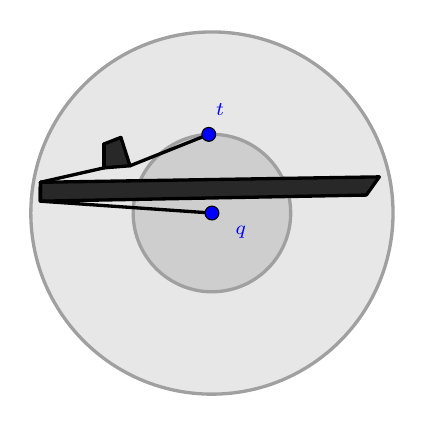
\begin{tikzpicture}[line cap=round,line join=round,>=triangle 45,x=1.0cm,y=1.0cm]
\definecolor{aqaqaq}{rgb}{0.6274509803921569,0.6274509803921569,0.6274509803921569}
\definecolor{qqqqff}{rgb}{0.,0.,1.}
\clip(1.6,0.47) rectangle (6.28,5.17);
\draw [line width=1.2pt,color=aqaqaq,fill=aqaqaq,fill opacity=0.3499999940395355] (3.9400050555577426,2.815716717828029) circle (1.cm);
\fill[line width=1.2pt,fill=black,fill opacity=1.0] (1.7619906352802,3.2064019550048823) -- (1.760948257574785,2.966272798087264) -- (5.9009925693289444,3.0440732742639014) -- (6.065992717197827,3.275305213897039) -- cycle;
\fill[line width=1.2pt,fill=black,fill opacity=1.0] (2.7838752248591803,3.776985670170509) -- (2.5711486339617498,3.69319853872332) -- (2.5711499019374466,3.389901746844879) -- (2.8995061535758593,3.4158740479215886) -- cycle;
\draw [line width=1.2pt,color=aqaqaq,fill=aqaqaq,fill opacity=0.25] (3.9400050555577426,2.815716717828029) circle (2.3cm);
\draw [line width=1.2pt] (1.7619906352802,3.2064019550048823)-- (1.760948257574785,2.966272798087264);
\draw [line width=1.2pt] (1.760948257574785,2.966272798087264)-- (5.9009925693289444,3.0440732742639014);
\draw [line width=1.2pt] (5.9009925693289444,3.0440732742639014)-- (6.065992717197827,3.275305213897039);
\draw [line width=1.2pt] (6.065992717197827,3.275305213897039)-- (1.7619906352802,3.2064019550048823);
\draw [line width=1.2pt] (2.7838752248591803,3.776985670170509)-- (2.5711486339617498,3.69319853872332);
\draw [line width=1.2pt] (2.5711486339617498,3.69319853872332)-- (2.5711499019374466,3.389901746844879);
\draw [line width=1.2pt] (2.5711499019374466,3.389901746844879)-- (2.8995061535758593,3.4158740479215886);
\draw [line width=1.2pt] (2.8995061535758593,3.4158740479215886)-- (2.7838752248591803,3.776985670170509);
\draw [line width=1.2pt] (3.9400050555577426,2.815716717828029)-- (1.760948257574785,2.9662727980872643);
\draw [line width=1.2pt] (1.760948257574785,2.9662727980872643)-- (1.7619906352802033,3.206401955004883);
\draw [line width=1.2pt] (1.7619906352802033,3.206401955004883)-- (2.5711499019374506,3.389901746844879);
\draw [line width=1.2pt] (2.8995061535758624,3.415874047921588)-- (3.8997931043534932,3.8149078902171505);
\begin{scriptsize}
\draw [fill=qqqqff] (3.9400050555577426,2.815716717828029) circle (2.5pt);
\draw[color=qqqqff] (4.30746415449908,2.57569402093485) node {$q$};
\draw [fill=qqqqff] (3.8997931043534932,3.8149078902171505) circle (2.5pt);
\draw[color=qqqqff] (4.042501567145657,4.1257251569523605) node {$t$};
\end{scriptsize}
\end{tikzpicture}
      \caption{
        \small recomputes the shortest path  
      }
      \label{edbt4}
    \end{subfigure}
  \end{subfigure}
  \caption{\small LVG algorithm}
\end{figure*}

Since $r>=d_o(q, t)$, when algorithm finish, it guarantees that no obstacle on current shortest
path, and thus proof the correctness. This algorithm can be extended to multi-target
scenario to solve OkNN problem:
\begin{itemize}
  \item Initially, $t$ is the \textit{k-th} nearest neighbor in Euclidean space, so that it
    guarantees that the VG always contains at least $k$ targets;
  \item Terminate when $r$  not less than the current \textit{k-th} nearest distance;
\end{itemize}

\subsection{Fast filter}

There's another similar work proposed by Xia\cite{xia2004fast},
the difference is, instead of considering obstacles in a circle area,
it only retrieves obstacles on current shortest path,
updates the LVG and recomputes the shortest path.
Since less obstacles are involved in VG,
the algorithm is called \textit{Fast Filter}.
Figure~\ref{xia} shows an example.
\begin{figure*}[!h]
  \centering
  \begin{subfigure}{.45\linewidth}
    \centering
    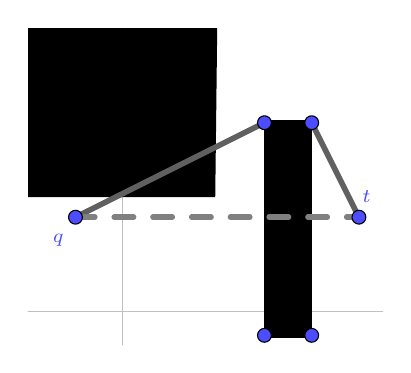
\begin{tikzpicture}[line cap=round,line join=round,>=triangle 45,x=0.6cm,y=0.6cm]
\definecolor{yqyqyq}{rgb}{0.5019607843137255,0.5019607843137255,0.5019607843137255}
\definecolor{wqwqwq}{rgb}{0.3764705882352941,0.3764705882352941,0.3764705882352941}
\definecolor{ududff}{rgb}{0.30196078431372547,0.30196078431372547,1.}
\definecolor{cqcqcq}{rgb}{0.7529411764705882,0.7529411764705882,0.7529411764705882}
\draw [color=cqcqcq,, xstep=4.0cm,ystep=4.0cm] (-2.,-0.7) grid (5.5,6.);
\clip(-2.,-0.7) rectangle (5.5,6.);
\fill[line width=2.pt,fill=black,fill opacity=1.0] (3.,4.) -- (3.,-0.5) -- (4.,-0.5) -- (4.,4.) -- cycle;
\fill[line width=2.pt,fill=black,fill opacity=1.0] (2.,6.) -- (1.958260850221742,2.42739675673013) -- (-2.036562862356449,2.42739675673013) -- (-2.,6.) -- cycle;
\draw [line width=2.pt] (3.,4.)-- (4.,4.);
\draw [line width=2.pt,color=wqwqwq] (4.,4.)-- (5.,2.);
\draw [line width=2.pt] (3.,-0.5)-- (4.,-0.5);
\draw [line width=2.pt,color=wqwqwq] (-1.,2.)-- (3.,4.);
\draw [line width=2.pt,dash pattern=on 7pt off 7pt,color=yqyqyq] (-1.,2.)-- (5.,2.);
\begin{scriptsize}
\draw [fill=ududff] (-1.,2.) circle (2.5pt);
\draw[color=ududff] (-1.3610221733554015,1.519358046860102) node {$q$};
\draw [fill=ududff] (5.,2.) circle (2.5pt);
\draw[color=ududff] (5.163642125127989,2.4314078950351963) node {$t$};
\draw [fill=ududff] (3.,4.) circle (2.5pt);
\draw [fill=ududff] (3.,-0.5) circle (2.5pt);
\draw [fill=ududff] (4.,-0.5) circle (2.5pt);
\draw [fill=ududff] (4.,4.) circle (2.5pt);
\end{scriptsize}
\end{tikzpicture}

    \caption{}
    \label{xia0}
  \end{subfigure}%
  \begin{subfigure}{.45\linewidth}
    \centering
    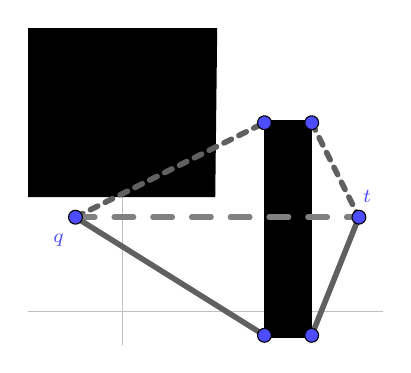
\begin{tikzpicture}[line cap=round,line join=round,>=triangle 45,x=.6cm,y=.6cm]
\definecolor{yqyqyq}{rgb}{0.5019607843137255,0.5019607843137255,0.5019607843137255}
\definecolor{wqwqwq}{rgb}{0.3764705882352941,0.3764705882352941,0.3764705882352941}
\definecolor{ududff}{rgb}{0.30196078431372547,0.30196078431372547,1.}
\definecolor{cqcqcq}{rgb}{0.7529411764705882,0.7529411764705882,0.7529411764705882}
\draw [color=cqcqcq,, xstep=4.0cm,ystep=4.0cm] (-2.,-0.7) grid (5.5,6.);
\clip(-2.,-0.7) rectangle (5.5,6.);
\fill[line width=2.pt,fill=black,fill opacity=1.0] (3.,4.) -- (3.,-0.5) -- (4.,-0.5) -- (4.,4.) -- cycle;
\fill[line width=2.pt,fill=black,fill opacity=1.0] (2.,6.) -- (1.958260850221742,2.42739675673013) -- (-2.036562862356449,2.42739675673013) -- (-2.,6.) -- cycle;
\draw [line width=2.pt] (3.,4.)-- (4.,4.);
\draw [line width=2.pt,dash pattern=on 3pt off 3pt,color=wqwqwq] (4.,4.)-- (5.,2.);
\draw [line width=2.pt,color=wqwqwq] (-1.,2.)-- (3.,-0.5);
\draw [line width=2.pt] (3.,-0.5)-- (4.,-0.5);
\draw [line width=2.pt,color=wqwqwq] (4.,-0.5)-- (5.,2.);
\draw [line width=2.pt,dash pattern=on 3pt off 3pt,color=wqwqwq] (-1.,2.)-- (3.,4.);
\draw [line width=2.pt,dash pattern=on 7pt off 7pt,color=yqyqyq] (-1.,2.)-- (5.,2.);
\begin{scriptsize}
\draw [fill=ududff] (-1.,2.) circle (2.5pt);
\draw[color=ududff] (-1.3607039979330486,1.5168391580998075) node {$q$};
\draw [fill=ududff] (5.,2.) circle (2.5pt);
\draw[color=ududff] (5.172498007716814,2.426820866029606) node {$t$};
\draw [fill=ududff] (3.,4.) circle (2.5pt);
\draw [fill=ududff] (3.,-0.5) circle (2.5pt);
\draw [fill=ududff] (4.,-0.5) circle (2.5pt);
\draw [fill=ududff] (4.,4.) circle (2.5pt);
\end{scriptsize}
\end{tikzpicture}

    \caption{}
    \label{xia1}
  \end{subfigure}
  \caption{
    \small Black polygons are obstacle,
    $q$ is query point, $t$ is the target.
    Initially, the VG only contains
    the rectangle obstacle between the $qt$,
    and the corresponding shortest path is computed (fig~\ref{xia0}).
    Then retrieves the square
    obstacle on the current path,
    updates VG and recomputes shortest path (fig~\ref{xia1}).
  }
  \label{xia}
\end{figure*}

To solve OkNN, we need following changes:
\begin{itemize}
  \item initially compute obstacle distance for k nearest neighbors, and store results in
    \textit{max-heap} with size $k$;
  \item keep retrieving next NN and compute the obstacle distance $d_o$;
  \item when $d_o$ not large than the top value of heap, pop top and insert the current $d_o$;
  \item terminate when the Euclidean distance to current NN is large than the Obstacle distance
    on top of the heap;
\end{itemize}
\subsection{Discussion}
When search space is large (e.g. target is far from the query point), \textit{fast
filter}\cite{xia2004fast} is
more efficient because it only consider obstacles that might on the path, meanwhile
\textit{LVG}\cite{zhang2004spatial} will build visibility graph for a large area, which is slow. 
In multi-target scenario, when $k$ is large, \textit{LVG}\cite{zhang2004spatial} is more efficient because
\textit{dijkstra} is a natural single-source algorithm, meanwhile, each time \textit{fast
filter}\cite{xia2004fast} can
only compute path for a single target, so that it duplicates effort for common prefixes of $k$
targets.

Both \textit{LVG}\cite{zhang2004spatial} and \textit{Fast filter}\cite{xia2004fast} are simple to understand,
provide optimality guarantees and the promise of fast performance. Such advantages make them
attractive to researchers and, despite more than a decade since their introduction,
they continue to appear as ingredients in a variety of kNN studies from the literature; e.g.
\cite{gao2011efficient,gao2016reverse}.
However, these visibility graph based algorithms also suffer from a number of notable
disadvantages including:
\begin{enumerate}[label=(\roman*)]
  \item costly online visibility checks;
  \item an incremental construction process that has up to quadratic space and time complexity for the worst case;
  \item duplicated effort, since the graph is discarded each time the query point changes.
\end{enumerate}

\section{Pathfinding on Navigation Mesh}\label{lrnav}

\subsection{Historic background}
Because of the limitation of VG, \textit{Navigation Mesh} comes to our sight.
Ronald first proposed this concept in 1986\cite{ronald1986pathfinding}, then it is applied on
robotics and game pathfinding.

Navigation mesh divides traversable space into convex polygons, the convexity of mesh
guarantees that all insides points are co-visible, so that it not needs visibility checking,
Figure~\ref{nav} shows an example.
Compare to VG (fig~\ref{vg}), it can be generated by\textit{Constrained Delaunay
Triangulation}\cite{chew1989constrained} in $O(nlogn)$ times,
so that it is feasible to preprocess the entire map.
Additionally, adding or removing obstacles only needs to modify a few number of mesh polygons,
which is very flexible. It seems like a perfect framework for OkNN,
the only problem is that how to compute obstacle distance on it.

\begin{figure}[htp]
  \centering
  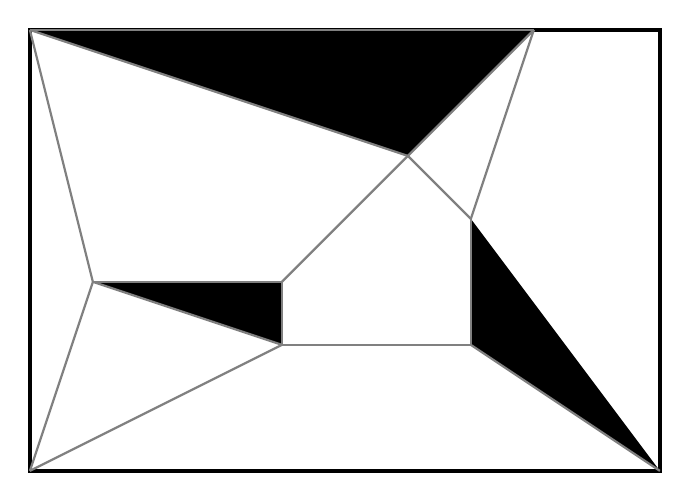
\begin{tikzpicture}[scale=0.8]
    %\coordinate (a) at (2, 6); 
\coordinate (a) at (0, 7);
\coordinate (b) at (8, 7); 
\coordinate (c) at (6, 5); 
\coordinate (d) at (1, 3);
\coordinate (e) at (4, 3);
\coordinate (f) at (4, 2);
\coordinate (g) at (7, 4);
\coordinate (h) at (7, 2);
%\coordinate (i) at (9, 0);
\coordinate (i) at (10, 0);
\coordinate (j) at (5, 2);
\coordinate (k) at (0, 7);
\coordinate (l) at (0, 0);
\coordinate (m) at (10, 0);
\coordinate (n) at (10, 7);
\coordinate (q) at (3, 4);
\coordinate (Q) at (3, 4);
\coordinate (t) at (9, 3);
\coordinate (o) at (7.5, 5.5);

\newcommand{\nodelabel}[2] {
    \node[fill,circle,scale=0.25,label=#2:$#1$,color=red] at (#1) {$#1$};
}

\newcommand{\medge}[2]{
    \draw[gray,thick] (#1)--(#2);
}

\newcommand{\vgedge}[2]{
    \draw[black,thick] (#1)--(#2);
}

\newcommand{\drawVs}{
    %\nodelabel{a}{above}
    \nodelabel{b}{below}
    \nodelabel{c}{below}
    
    %\nodelabel{d}{left}
    \nodelabel{e}{right}
    \nodelabel{f}{below}
    
    \nodelabel{g}{above}
    \nodelabel{h}{below}
    %\nodelabel{i}{below}
}

\newcommand{\drawmeshs}{
    \medge{a}{k},\medge{a}{d},\medge{a}{b},\medge{a}{c}
    \medge{b}{c},
    \medge{c}{g}
    \medge{d}{f},\medge{d}{l},\medge{d}{e}
    \medge{l}{f}
    \medge{e}{c},\medge{e}{f}
    \medge{f}{h}
    \medge{g}{h},\medge{g}{b}
    \medge{h}{i}
}

\newcommand{\drawobstacles}{
    \fill[black] (a)--(b)--(c)--cycle;
    \fill[black] (g)--(h)--(i)--cycle;
    \fill[black] (d)--(e)--(f)--cycle;
}

\newcommand{\drawstart} {
    % \fill[blue] (q) circle[radius=.5ex];
    % \node[above] at (q) {$q$};
    \node[fill,circle,scale=0.25,label=above:$q$,color=blue] at (q) {$q$};

}

\newcommand{\drawend}{
    \fill[blue] (t) circle[radius=.5ex];
    \node[above] at (t) {$t$};
}

\newcommand{\drawboundary}{
    \draw[black, ultra thick] (k)--(n)--(m)--(l)--cycle;
}

\newcommand{\showvisible} {
    \fill[lightgray] (c)--(e)--(d)--(a);
    \nodelabel{e}{right}
    \nodelabel{c}{below}
    \drawstart;
}

\newcommand{\stepa} {
    \fill[lightgray] (c)--(e)--(d)--(a);
    \fill[lightgray] (c)--(g)--(h)--(f)--(e);
    \draw[black, thin] (q)--(g);
    \draw[green, very thick] (e)--(c);
    \drawstart
    \drawVs
}

\newcommand{\stepb} {
    \fill[lightgray] (c)--(e)--(d)--(a);
    \fill[lightgray] (c)--(g)--(h)--(f)--(e);
    \fill[lightgray] (c)--(g)--(b);
    \draw[black, thin] (q)--(g);
    \draw[green, very thick] (e)--(c);
    \draw[black, thin] (g)--(t);
    \draw[black, thin] (q)--(g);
    \draw[green, very thick] (g)--(c);
    \draw[green, very thick] (g)--(b);
    \drawstart
    \drawend
    \drawVs
}

\newcommand{\polyanyaexpand}{
    \draw[black,very thin, dashed] (q)--($(q)!5cm!(e)$);
    \draw[black,very thin, dashed] (q)--($(q)!5cm!(c)$);
    \draw[orange!50, line width=3pt] (j)--(h);
    \draw[orange!50, line width=3pt] (h)--(g);
    \draw[orange!50, line width=3pt] (g)--(c);
    \draw[cyan, line width=3pt] (e)--(f);
    \draw[cyan, line width=3pt] (f)--(j);
}

\newcommand{\drawVG}{
    \vgedge{a}{d},\vgedge{a}{e},\vgedge{a}{g},\vgedge{a}{h}
    \vgedge{b}{g},\vgedge{b}{m}
    \vgedge{c}{d},\vgedge{c}{e},\vgedge{c}{g},\vgedge{c}{f},\vgedge{c}{h}
    \vgedge{d}{l},\vgedge{d}{g}
    \vgedge{e}{h},\vgedge{e}{n}
    \vgedge{f}{l},\vgedge{f}{h},\vgedge{f}{m}
    \vgedge{g}{n}
}
\newcommand{\drawmap}{
    \drawboundary
    \drawobstacles
    \drawmeshs
    \drawVs
    \drawstart
    \drawend
}

\newcommand{\intervalexpansion}{
    \drawboundary
    \drawobstacles
    \drawmeshs
    {\draw[green!50, line width=3pt, dashed] (e)--(d);}
    {\draw[green!50, line width=3pt, dashed] (d)--(a);}
    {\draw[green!50, line width=3pt, dashed] (a)--(c);}
    {\draw[green!50, line width=3pt, dashed] (e)--(c);}
    {\draw[green!50, line width=3pt, dashed] (d)--(l);}
    {\draw[green!50, line width=3pt, dashed] (e)--(f);}
    {\draw[green!50, line width=3pt, dashed] (f)--(j);}
    {\draw[green!50, line width=3pt, dashed] (j)--(h);}
    {\draw[green!50, line width=3pt, dashed] (g)--(h);}
    {\draw[green!50, line width=3pt, dashed] (c)--(g);}
    {\draw[green!50, line width=3pt, dashed] (g)--(b);}
    {\draw[black, line width=3pt] (q)--(g);}
    {\draw[black, line width=3pt] (g)--(t);}
    \drawstart
    \drawend 
    \drawVs
}

    {
    \drawboundary
    \drawobstacles
    \drawmeshs
    }
  \end{tikzpicture}
  \caption{\small Navigation Mesh: The rectangle is the boundary of the map, black polyogns are
  obstacles, gray lines are edges of mesh polygons.}
  \label{nav}
\end{figure}

Previous pathfinding algorithms on navigation mesh are not suitable for spatial query
processing, and thus it's not attractive to researchers in this fields.
Three widly used algorithms are:
\begin{itemize}
\item Channel Search \cite{kallmann2005path}: first find an abstract path from start to target
    composed by polygons, then refine the abstract path to a sequence of concrete points. This
    algorithm only generate an approximately shortest path, the lack of optimality makes it not
    suitable for OkNN query.
  \item TA* \cite{demyen2006efficient}: similar to Channel Search, but it can repeat the search
    process until finding an optimal shortest path. The repeating is time-consuming, so it is not
    suitable for query processing.
  \item TRA* \cite{demyen2006efficient}: similar to TA*, but TRA* can utilize preprocessing to
    speed up pathfinding. The problem is that the precomputed information will be invalid when
    environment change, so it is not suitable for database scenario.
\end{itemize}

However, this fact has been changed by a recent work called
\textit{Polyanya}\cite{cuicompromise}. It is a fast, optimal and fexible pathfinding algorithm
which is perfect for query processing in spatial database.

\subsection{Polyanya}
\textit{Polyanya} can be seen as an instance of \textit{A*}: it performs a best-first search
using an admissible heuristic function to prioritise nodes. The mechanical details are however
quite different, there are three key components:
\begin{itemize}
\item \textbf{Search Nodes}: Conventional  search algorithms proceed from one traversable point
  to the next. \textit{Polyanya}, by comparison, searches from one \textit{edge} of the
  navigation mesh to another. In this model, search nodes are tuples $(I, r)$ where each
  $I=[a,b]$ is a contiguous interval of points and $r$ is a distinguished point called the
  \textit{root}. Nodes are constructed such that each point $p \in I$ is visible from $r$.
  Meanwhile, $r$ itself corresponds to the last turning point on the path: from $q$ to any $p
  \in I$. Figure~\ref{snode} shows an example.

  \begin{figure}[htb]
    \centering
     %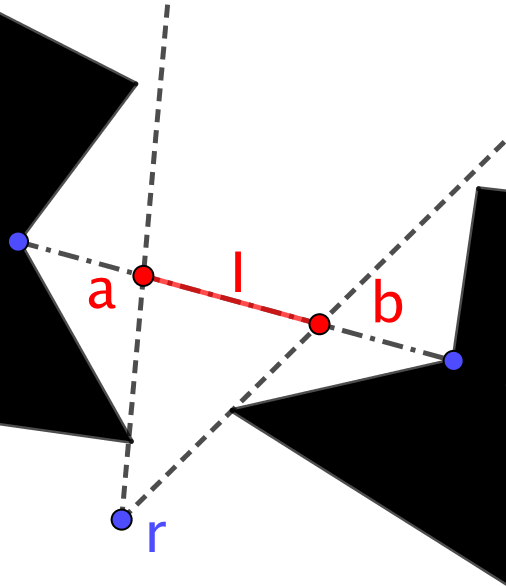
\includegraphics[width=.5\linewidth]{pic/snode.png}
    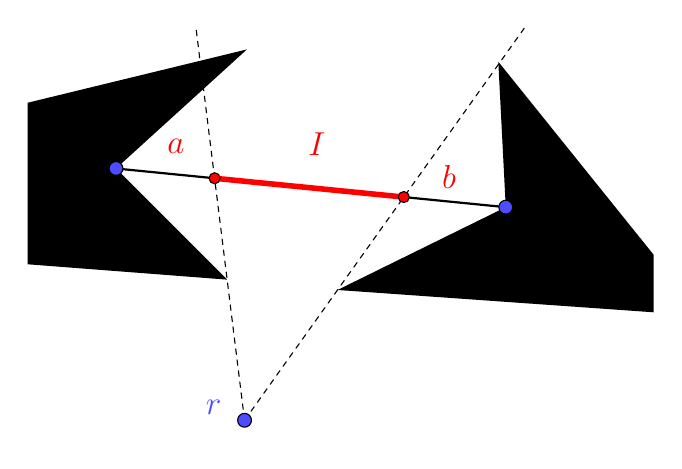
\begin{tikzpicture}[line cap=round,line join=round,>=triangle 45,x=1.5cm,y=1.5cm]
\definecolor{ffqqqq}{rgb}{1.,0.,0.}
\definecolor{ududff}{rgb}{0.30196078431372547,0.30196078431372547,1.}
\clip(-0.8,-1.6) rectangle (4.5,1.9);
\fill[line width=2.pt,fill=black,fill opacity=1.0] (1.0568852561643571,1.7160911807341181) -- (-0.05223307140302057,0.7078017920365031) -- (0.8888370247147546,-0.23326830408127103) -- (-0.8588645823611135,-0.09882971892158902) -- (-0.8084501129262327,1.2623609558201914) -- cycle;
\fill[line width=2.pt,fill=black,fill opacity=1.0] (1.823359787139688,-0.3207843311089217) -- (3.2477722134398506,0.38019461763527085) -- (3.1845504618814697,1.6117703305615074) -- (4.915447245812395,-0.5392470319934045) -- cycle;
\draw [thick] (-0.05223307140302057,0.7078017920365031)-- (3.2477722134398506,0.38019461763527085);
\draw [dash pattern=on 2pt off 2pt,domain=-0.8:1.0362283883022219] plot(\x,{(-1.0239487358475874--1.1906912514220491*\x)/-0.1473913635874673});
\draw [dash pattern=on 2pt off 2pt,domain=1.0362283883022219:4.5] plot(\x,{(-2.2639847616004545--1.1031752243943984*\x)/0.7871313988374662});
\draw [line width=2.pt,color=ffqqqq] (2.3846562728722773,0.4658802302519392)-- (0.7826045650521551,0.6249235007746435);
\begin{scriptsize}
\draw [fill=ududff] (-0.05223307140302057,0.7078017920365031) circle (2.5pt);
\draw [fill=ududff] (3.2477722134398506,0.38019461763527085) circle (2.5pt);
\draw [fill=ududff] (1.0362283883022219,-1.4239595555033202) circle (2.5pt);
\draw[color=ududff] (0.7743350405885554,-1.3148373272892926) node {\large $r$};
\draw [fill=ffqqqq] (2.3846562728722773,0.4658802302519392) circle (2.0pt);
\draw[color=ffqqqq] (2.767634409298129,0.6348131501346688) node {\large $b$};
\draw [fill=ffqqqq] (0.7826045650521551,0.6249235007746435) circle (2.0pt);
\draw[color=ffqqqq] (0.45424317116074064,0.8967064978483352) node {\large $a$};
\draw[color=ffqqqq] (1.6473128663007772,0.9112561282768722) node {\large $I$};
\end{scriptsize}
\end{tikzpicture}

    \caption{\small Search nodes in Polyanya. Notice that the interval $I = [a, b]$ is
    a contiguous subset of points drawn from an edge of the navigation mesh.
    The corresponding root point, $r$, is either the query point itself 
    or the vertex of an obstacle. Taken together they form the search node $(I, r)$.}
    \label{snode}
  \end{figure}

\item \textbf{Successors}: Successor nodes $(I', r')$ are generated by "pushing" the current
  interval $I$ away from its root $r$ and throught the interior of an adjacent and traversable
  polygon. A successor is said to be \textit{obervable} if each point $p' \in I'$ is visible
  from $r$. The successor node in this case is formed by the tuple $(I',r)$. By contrast, a
  successor is said to be \textit{non-observable} if the \textit{taut} (i.e. locally optimal)
  path from $r$ to each $p' \in I'$ must pass through one of the endpoints of current interval
  $I=[a,b]$. The successor node in this case is formed by the tuple $(I', r')$ with $r'$ as
  one of the points $a$ or $b$. Figure~\ref{suc} shows an example.
 
  Note that the target point is inserted in the open list as a special case
  (observable or non-observable) successor whenever the search reaches its 
  containing polygon.  The interval of this successor contains only the target.
  \begin{figure}[ht]
    \centering
    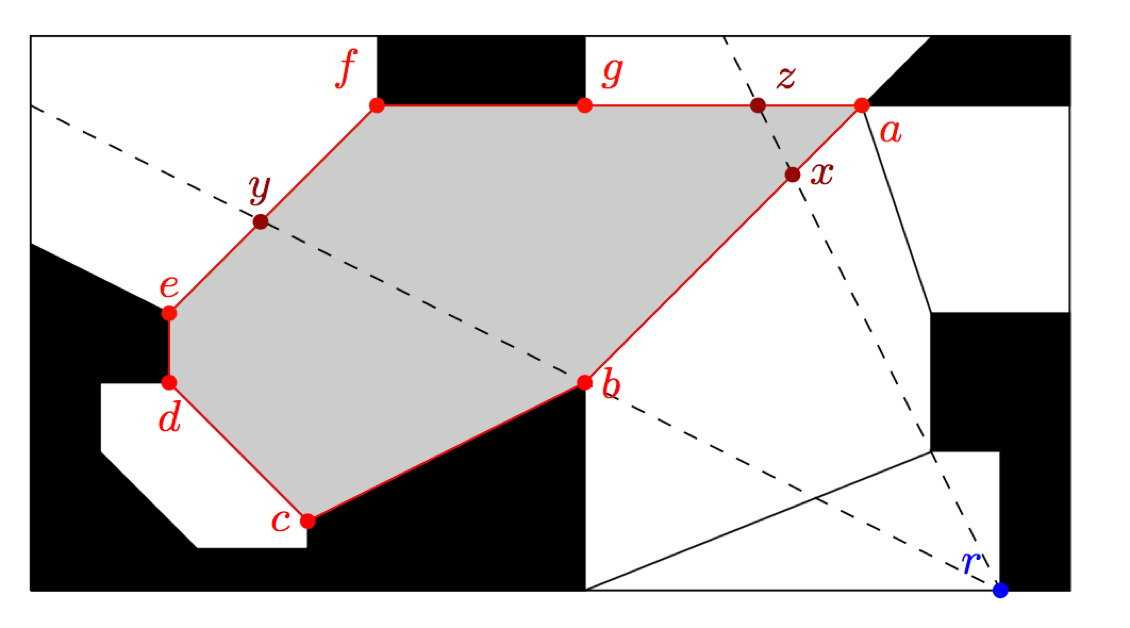
\includegraphics[width=.6\linewidth]{pic/suc.png}
    \caption{\small 
    From \cite{cuicompromise}. We expand the node $([b,x],r)$ which has
    $([z,g],r)$ and $([f,y],r)$ as observable successors.
    In addition, the nodes $([c,d],b)$, $([d,e],b)$ and $([e,y],b)$ 
    are non-observable. All other potential 
    successors can be safely pruned (more details in~\cite{cuicompromise}).}
    \label{suc}
  \end{figure}

\item \textbf{Evaluation}: When prioritising nodes for expansion, \textit{Polyanya} makes use of an
  \textit{f-value} estimation function which bounds the length of the optimal path:
  from $q$, throught the current node (i.e. via some $p \in I$) and onto the target. There are
  three cases to consider which describe the relative positions of the target in relation to
  the current node. These are illustrated in Figure~\ref{ef}. The objective in each case is to
  choose the unique $p \in I$ that minimise the estimate. The three cases together are
  sufficient to guarantee that the estimator is admissible.

  \begin{figure}[htp]
    \centering
    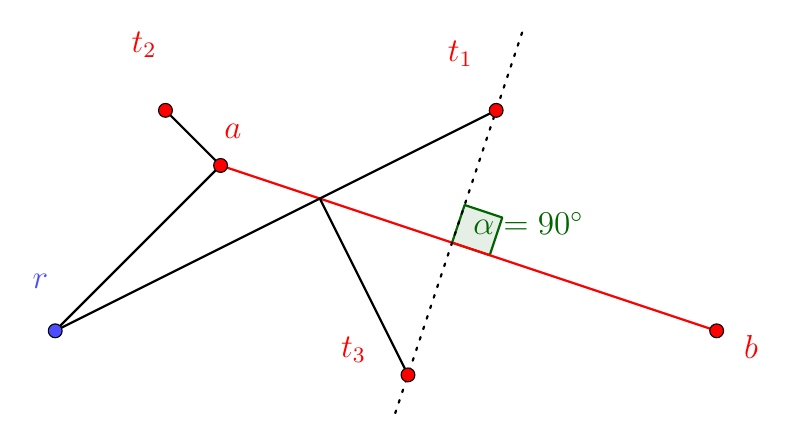
\begin{tikzpicture}[line cap=round,line join=round,>=triangle 45,x=.7cm,y=.7cm]
\newcommand{\degre}{\ensuremath{^\circ}}
\definecolor{qqwuqq}{rgb}{0.,0.39215686274509803,0.}
\definecolor{ududff}{rgb}{0.30196078431372547,0.30196078431372547,1.}
\definecolor{ffqqqq}{rgb}{1.,0.,0.}
\definecolor{cqcqcq}{rgb}{0.7529411764705882,0.7529411764705882,0.7529411764705882}

%\draw [color=cqcqcq,, xstep=2.0cm,ystep=2.0cm] (-2.5,-1.5) grid (11.1,5.5);
\clip(-2.5,-1.5) rectangle (11.1,5.5);
\draw [thick,color=qqwuqq,fill=qqwuqq,fill opacity=0.10000000149011612] (5.882794718512914,1.3724017604956955) -- (6.1103929580172185,2.0551964790086092) -- (5.427598239504305,2.282794718512914) -- (5.2,1.6) -- cycle; 
\draw [thick,color=ffqqqq] (1.,3.)-- (10.,0.);
\draw [thick,dash pattern=on 1pt off 3pt,domain=-2.5:11.1] plot(\x,{(-42.--9.*\x)/3.});
\draw [thick] (-2.,0.)-- (1.,3.);
\draw [thick] (1.,3.)-- (0.,4.);
\draw [thick] (-2.,0.)-- (6.,4.);
\draw [thick] (4.4,-0.8)-- (2.8,2.4);
\begin{scriptsize}
\draw [fill=ffqqqq] (1.,3.) circle (2.5pt);
\draw[color=ffqqqq] (1.2251463573152723,3.6132615238618353) node {\large $a$};
\draw [fill=ffqqqq] (10.,0.) circle (2.5pt);
\draw[color=ffqqqq] (10.623297185327285,-0.2884978451684127) node {\large $b$};
\draw [fill=ududff] (-2.,0.) circle (2.5pt);
\draw[color=ududff] (-2.269472903642263,0.8989941367103583) node {\large $r$};
\draw [fill=ffqqqq] (0.,4.) circle (2.5pt);
\draw[color=ffqqqq] (-0.3864499038059212,5.190929442643631) node {\large $t_2$};
\draw [fill=ffqqqq] (6.,4.) circle (2.5pt);
\draw[color=ffqqqq] (5.347439951551588,5.021287730946663) node {\large $t_1$};
\draw[color=qqwuqq] (6.585824446939453,1.9507727492315556) node {\large $\alpha = 90\textrm{\degre}$};
\draw [fill=ffqqqq] (4.4,-0.8) circle (2.5pt);
\draw[color=ffqqqq] (3.413524438206156,-0.3393903586775029) node {\large $t_3$};
\end{scriptsize}
\end{tikzpicture}

    \caption{\small
    Polyanya $f$-value estimator. The current node is $(I, r)$ with $I = [a, b]$ and
    each of $t_1, t_2, t_3$ are possible target locations.
    \textbf{Case 1}: the target is $t_1$. In this case the point $p \in I$ with minimum
    $f$-value is at the intersection of the interval $I$ and the line $r \rightarrow t_1$.
    \textbf{Case 2}: the target is $t_2$. In this case the $p \in I$ with minimum $f$-value
    is one of two endpoints of $I$. 
    \textbf{Case 3}: the target is $t_3$. In this case the $p \in I$ with minimum $f$-value
    is obtained by first mirroring $t_3$ through $[a, b]$ and applying Case 1 or Case 2
    to the mirrored point (here, $t_1$). Notice that in this case, simply $r$ to $t_3$
    doesn't give us the \textit{h-value}, based on definition, it must reach the interval
    first.
    }
  \label{ef}
  \end{figure}
\end{itemize}

Similar to \textit{A*}, \textit{Polyanya} terminates when the target is expanded or when the
open list is empty. Extending it to multi-target OkNN is not a trivial problem, we will discuss
this in chapter~\ref{proposedalgo}.

\section{Other Obstacle Spatial Queries}\label{lrquery}
Obstacle spatial query processing is a broad research area, and many existing works are still
based on visibility graph, in this section, we review those works which can get benefit from
OkNN in our research. 

\begin{itemize}

\item \textbf{Obstacle Range Query}(OR): given query point $q$ and range $r$,
  it returns all targets which obstacle distance to $q$ are less or equal to $r$ \cite{zhang2004spatial}. 
To solve this by OkNN, we can let $k$ be infinite and terminate the algorithm when current
obstacle distance large than $r$.

\item \textbf{Obstacle Reverse k-Nearest Neighbor}(ORkNN): it is proposed by Gao in
2011\cite{gao2011efficient} for $k=1$, and be generalized to $k>1$ in
2016\cite{gao2016reverse}. ORkNN given query point $q$ and $k$, return a set of target which
regards $q$ as its OkNN: $\{t | q \in OkNN(t, k)\}$. The query processing has two stages:
(i) \textit{search stage}: explore search space to get a set of candidate; (ii) \textit{refine
stage}: calls OkNN for each candidate, remove a candidate if $q$ is not its OkNN.
The first stage needs to compute obstacle distance to prune search space, and the second stage 
can directly get benefit from the improvement of OkNN.

\item \textbf{Continuous Obstacle k-Nearest Neighbor}(COkNN): it's proposed in
  2009\cite{gao2009continuous}, simliar to OkNN, but the query becomes a segment.
  The algorithm first generates a list of "split" points, and reduce the problem to finding the
    OkNN for these points. It also needs to compute obstacle distance to prune search space.

\end{itemize}

\section{Summary}
In this chapter, we review works which related to our research, basically they are in three
fields: Spatial Index, Spatial Query Processing and AI Pathfinding. The major finding is that,
in OkNN problem, existing VG based algorithms are hard to improve, so we look for a new
framework, meanwhile, the new work in AI Pathfinding field shows us a new direction.
Such finding inspires us to proposed our research problem: an OkNN algorithm on navigation mesh.
We will discuss more detail about this in chapter~\ref{proposedalgo}.

\chapter{Proposed Algorithms}\label{proposedalgo}
\section{Overview}\label{proposedoverview}
From the previous chapter, we have introduced a very fast point-to-point algorithm \textit{Polyanya}, 
in this chapter, we discuss how to effectively adapt \textit{Polyanya} for OkNN settings where
there are multiple candidate targets. In section~\ref{prob}, we introduce formal problem
statement and math notations; in section~\ref{mot}, we introduce two less efficient but very
straightforward solution to show the motivations of our proposed research;
section~\ref{intervalh} and \ref{targeth} present our research works which discuss the design of our algorithms and the correctness in theory.

\section{Problem Statement}\label{prob}
OkNN is a spatial query in two dimensions that can be formalised as follows:
\begin{definition}{Obstacle k-Nearest Neighbour (OkNN):}\newline
Given a set of points $T$, a set of obstacles $O$, a distinguished point $q$ and and an integer $k$: 
\textbf{return} a set $\text{kNN} = \{t | t \in T\}$ such that $d_o(q, t) \le d_o(q, t_k)$ for all $t \in \text{kNN}$.
\end{definition}

\noindent Where:
\begin{itemize}[leftmargin=+1cm]
\item $O$ is a set of non-traversable polygonal obstacles.
\item $T$ is a set of traversable points called \emph{targets}.
\item $q$ is a traversable point called the \emph{query point}.
\item $k$ is an input parameter that controls the number of nearest neighbours that will be returned.
\item $d_e$ and $d_o$ are functions that measure the shortest distance between two points, as discussed below.
\item $t_k$ is the $k^{th}$ nearest neighbour of $q$.
\item $h_p(n, t)$ is the \textit{h-value} in Polyanya for a given search node $n$ and a target
  $t$.
\item $h_v(n)$ is the \textit{h-value} in Interval Heuristic for a given search node $n$.
\item $h_t(n)$ is the \textit{h-value} in Target Heuristic for a given search node $n$.
\end{itemize}
\noindent
Stated in simple words, the objective is to find the set of $k$ targets which are closest to $q$ from among all possible candidates in $T$.
When discussing distances between two points $q$ and $t$ we distinguish between two metrics:
$d_e(q, t)$ which is the well known Euclidean metric (i.e. ``straight-line distance'')
and $d_o(q, t)$ which measures the length of a shortest path $\pi_{q, t} = \langle q, \ldots, t\rangle$ between points $q$ and $t$ such that
no pairwise segment of the path intersects any point inside an obstacle (i.e. ``obstacle avoiding distance'').


\section{Motivation}\label{mot}
Since \textit{Polyanya} instantiates \textit{A*} search and since that algorithm is itself a
special case of \textit{Dijkstra}'s well know technique, there exists a simple modification at
hand: we can simply remove the influence of the cost-to-go heuristic and allow the search to
continue until it has expanded the $k^{th}$ target, let's call this \textbf{\textit{zero-heuristic}}.
All other aspects of the algorithm, including termination
\footnote{There are two cases to consider depending on whether the query and target points are in the same polygon or in different polygons.
Both are described in~\cite{cuicompromise}}, remain unchanged.

\begin{figure}[ht]
    \centering
    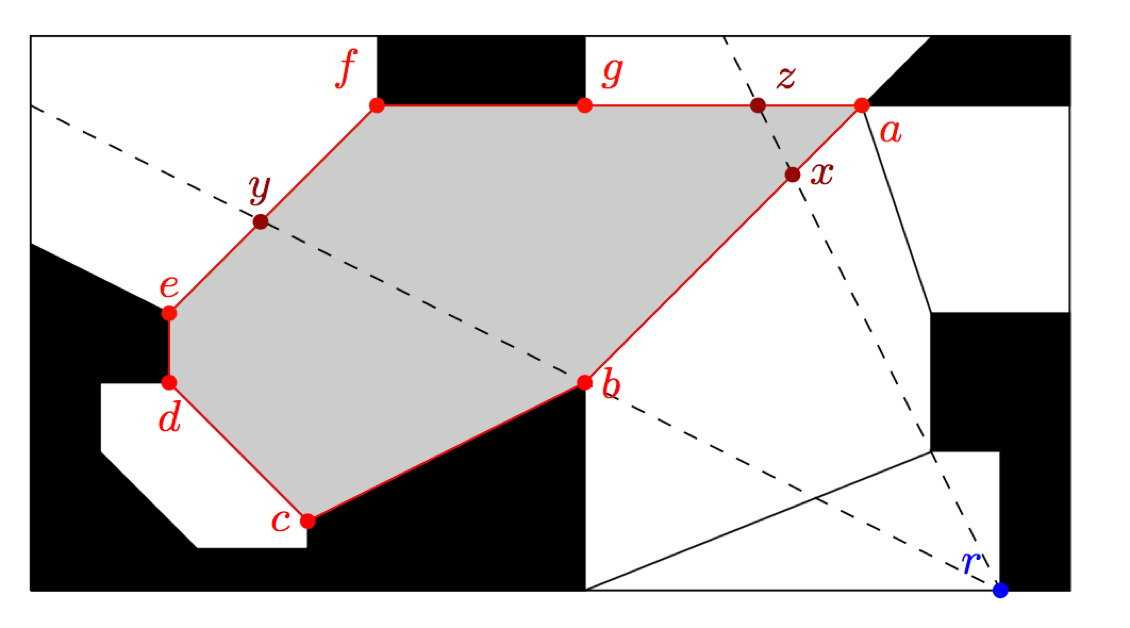
\includegraphics[width=.6\linewidth]{pic/suc.png}
    \caption{\small Example of successors from \cite{cuicompromise}.}
    \label{suc2}
\end{figure}

The version of \textit{Polyanya} we have just described is unlikely to be efficient. Without a
heuristic function for guidance, nodes can only be prioritized by the \textit{g-value} of their
root point, which is settled at the time of expansion. However, the \textit{g-value} does not
reflect the distance between the root and its corresponding interval. For example, in
Figure~\ref{suc2}, all observable successors would have the same expansion priority. Thus we
may expand many nodes, all equally priomising but having distant intervals, and all before
reaching a nearby target node with a slightly higher \textit{g-value}.

Another naive adaption is repeatedly calling an unmodified point-to-point \textit{Polyanya}
search, from the query point and to each target, let's call this \textbf{\textit{brute-force
Polyanya}}, see in algorithm~\ref{brute}. It is obvious that this solution is
inefficient when targets are many, however, in chapter\ref{empirical} we will see it
outperforms other proposed algorithms in certain contexts. 
\begin{algorithm}[!htp]
  \input{./code/brute_polyanya.pseudo}
  \caption{Brute-force Polyanya}
  \label{brute}
\end{algorithm}
To deal with this problem we develop two online heuristics which can be fruitfully applied to OkNN:
\begin{itemize}
  \item The Interval Heuristic, which prioritizes nodes using the closest point from its
    associated interval.
  \item The Target Heuristic, which relies on a Euclidean nearest neighbour estimator to
    provide a target dynamically at the time of expansion.
\end{itemize}
Each of these heuristic is applied in the usual way compute a final expansion priority: 
$f(n) = \textit{g-value}(n) + \textit{h-value}(n)$. In the remainder of this chapter we explore
these ideas in turn.

\section{Interval Heuristic}\label{intervalh}
In some OkNN settings targets are myriad and one simply requires a fast algorithm to explore
the local area. This approach is in contrast to more sophisticated methods which apply spatial
reasoning to prune the set of candidates. The idea we introduce for such settings is simple and
can be formalised as follows:

\begin{definition}
  Given search node $(I, r)$, the Interval Heuristic computes a value $h_i(I, r)$ which
  is the minimal Euclidean distance from the root $r$ to the segment $I$.
\end{definition}

Applying the Interval Heuristic $h_i$ requires solving a simple geometric problem: finding the
closest point on a line. The operation has low constant time complexity and we apply
standard techniques. Algorithm~\ref{intervalsrc} shows an example.

\begin{algorithm}[!htb]
  \input{./code/interval.pseudo}
  \caption{Polyanya OkNN with interval heuristic}
  \label{intervalsrc}
\end{algorithm}

\begin{theorem}{\textbf{(consistency)}:}\label{nodesc}
  The $\textit{f-value}$ of successor node is not less than the $\textit{f-value}$ of the parent
  search node.
\end{theorem}

\begin{proof}
  Using the interval heuristic, when the successor is a search node, its \textit{f-value}
  can be interpreted as a lower-bound of the length of path from
  $s$ to any point on the segment $I$ through root $r$, and since it is generated by pushing
  away from the parent search node, its \textit{f-value} is larger than \textit{f-value}
  of the parent search node. If successor is a target node, the \textit{f-value} is the the length
  of the corresponding path and not less than the parent search node (the two values are equal 
  when the target is on the segment $I$).%$\square$
\end{proof}

\begin{corollary}
  Expanding a target node corresponds to finding a shortest path.
\end{corollary}

\begin{proof}
  As per Theorem~\ref{nodesc}, when a final node is expanded there exists
  no remaining candidate on the open list which can reach the node with a smaller $f$-value.
\end{proof}

\section{Target Heuristic}\label{targeth}
In some OkNN settings the set of target are few (i.e. sparse), or there is a filter on the
query, for example, the query is like "the nearest storage location where capacity $>=100$". 
In these cases, without a reasonable heuristic guide, it is possible to perform many redundant
expansions in areas where no nearest neighbor can exist, Figure~\ref{hv} shows an example. 
\begin{figure}[htp]
  \centering
  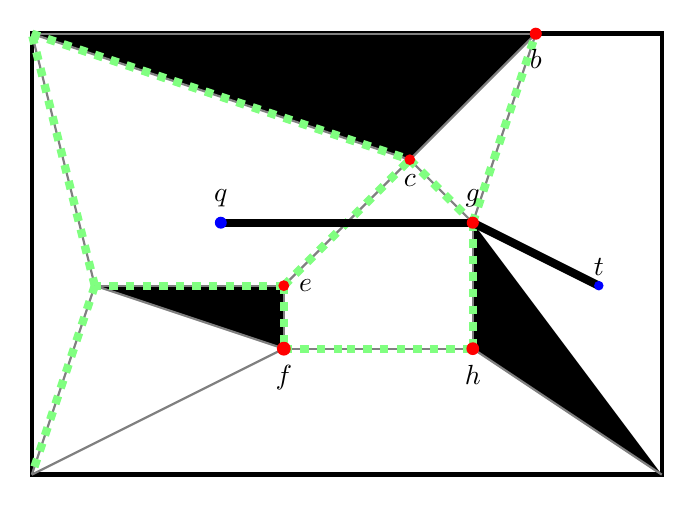
\begin{tikzpicture}[scale=0.8]
    %\coordinate (a) at (2, 6); 
\coordinate (a) at (0, 7);
\coordinate (b) at (8, 7); 
\coordinate (c) at (6, 5); 
\coordinate (d) at (1, 3);
\coordinate (e) at (4, 3);
\coordinate (f) at (4, 2);
\coordinate (g) at (7, 4);
\coordinate (h) at (7, 2);
%\coordinate (i) at (9, 0);
\coordinate (i) at (10, 0);
\coordinate (j) at (5, 2);
\coordinate (k) at (0, 7);
\coordinate (l) at (0, 0);
\coordinate (m) at (10, 0);
\coordinate (n) at (10, 7);
\coordinate (q) at (3, 4);
\coordinate (Q) at (3, 4);
\coordinate (t) at (9, 3);
\coordinate (o) at (7.5, 5.5);

\newcommand{\nodelabel}[2] {
    \node[fill,circle,scale=0.25,label=#2:$#1$,color=red] at (#1) {$#1$};
}

\newcommand{\medge}[2]{
    \draw[gray,thick] (#1)--(#2);
}

\newcommand{\vgedge}[2]{
    \draw[black,thick] (#1)--(#2);
}

\newcommand{\drawVs}{
    %\nodelabel{a}{above}
    \nodelabel{b}{below}
    \nodelabel{c}{below}
    
    %\nodelabel{d}{left}
    \nodelabel{e}{right}
    \nodelabel{f}{below}
    
    \nodelabel{g}{above}
    \nodelabel{h}{below}
    %\nodelabel{i}{below}
}

\newcommand{\drawmeshs}{
    \medge{a}{k},\medge{a}{d},\medge{a}{b},\medge{a}{c}
    \medge{b}{c},
    \medge{c}{g}
    \medge{d}{f},\medge{d}{l},\medge{d}{e}
    \medge{l}{f}
    \medge{e}{c},\medge{e}{f}
    \medge{f}{h}
    \medge{g}{h},\medge{g}{b}
    \medge{h}{i}
}

\newcommand{\drawobstacles}{
    \fill[black] (a)--(b)--(c)--cycle;
    \fill[black] (g)--(h)--(i)--cycle;
    \fill[black] (d)--(e)--(f)--cycle;
}

\newcommand{\drawstart} {
    % \fill[blue] (q) circle[radius=.5ex];
    % \node[above] at (q) {$q$};
    \node[fill,circle,scale=0.25,label=above:$q$,color=blue] at (q) {$q$};

}

\newcommand{\drawend}{
    \fill[blue] (t) circle[radius=.5ex];
    \node[above] at (t) {$t$};
}

\newcommand{\drawboundary}{
    \draw[black, ultra thick] (k)--(n)--(m)--(l)--cycle;
}

\newcommand{\showvisible} {
    \fill[lightgray] (c)--(e)--(d)--(a);
    \nodelabel{e}{right}
    \nodelabel{c}{below}
    \drawstart;
}

\newcommand{\stepa} {
    \fill[lightgray] (c)--(e)--(d)--(a);
    \fill[lightgray] (c)--(g)--(h)--(f)--(e);
    \draw[black, thin] (q)--(g);
    \draw[green, very thick] (e)--(c);
    \drawstart
    \drawVs
}

\newcommand{\stepb} {
    \fill[lightgray] (c)--(e)--(d)--(a);
    \fill[lightgray] (c)--(g)--(h)--(f)--(e);
    \fill[lightgray] (c)--(g)--(b);
    \draw[black, thin] (q)--(g);
    \draw[green, very thick] (e)--(c);
    \draw[black, thin] (g)--(t);
    \draw[black, thin] (q)--(g);
    \draw[green, very thick] (g)--(c);
    \draw[green, very thick] (g)--(b);
    \drawstart
    \drawend
    \drawVs
}

\newcommand{\polyanyaexpand}{
    \draw[black,very thin, dashed] (q)--($(q)!5cm!(e)$);
    \draw[black,very thin, dashed] (q)--($(q)!5cm!(c)$);
    \draw[orange!50, line width=3pt] (j)--(h);
    \draw[orange!50, line width=3pt] (h)--(g);
    \draw[orange!50, line width=3pt] (g)--(c);
    \draw[cyan, line width=3pt] (e)--(f);
    \draw[cyan, line width=3pt] (f)--(j);
}

\newcommand{\drawVG}{
    \vgedge{a}{d},\vgedge{a}{e},\vgedge{a}{g},\vgedge{a}{h}
    \vgedge{b}{g},\vgedge{b}{m}
    \vgedge{c}{d},\vgedge{c}{e},\vgedge{c}{g},\vgedge{c}{f},\vgedge{c}{h}
    \vgedge{d}{l},\vgedge{d}{g}
    \vgedge{e}{h},\vgedge{e}{n}
    \vgedge{f}{l},\vgedge{f}{h},\vgedge{f}{m}
    \vgedge{g}{n}
}
\newcommand{\drawmap}{
    \drawboundary
    \drawobstacles
    \drawmeshs
    \drawVs
    \drawstart
    \drawend
}

\newcommand{\intervalexpansion}{
    \drawboundary
    \drawobstacles
    \drawmeshs
    {\draw[green!50, line width=3pt, dashed] (e)--(d);}
    {\draw[green!50, line width=3pt, dashed] (d)--(a);}
    {\draw[green!50, line width=3pt, dashed] (a)--(c);}
    {\draw[green!50, line width=3pt, dashed] (e)--(c);}
    {\draw[green!50, line width=3pt, dashed] (d)--(l);}
    {\draw[green!50, line width=3pt, dashed] (e)--(f);}
    {\draw[green!50, line width=3pt, dashed] (f)--(j);}
    {\draw[green!50, line width=3pt, dashed] (j)--(h);}
    {\draw[green!50, line width=3pt, dashed] (g)--(h);}
    {\draw[green!50, line width=3pt, dashed] (c)--(g);}
    {\draw[green!50, line width=3pt, dashed] (g)--(b);}
    {\draw[black, line width=3pt] (q)--(g);}
    {\draw[black, line width=3pt] (g)--(t);}
    \drawstart
    \drawend 
    \drawVs
}

    \intervalexpansion
  \end{tikzpicture}
  \caption{\small Search space of Interval Heuristic:$q$ is query point,
  $t$ is a target, green dashed segments are the interval of expanded search nodes.
  From the figure we can see that the algorithm does unnecessary expansions in the direction that no target.}
  \label{hv}
\end{figure}
\noindent
In such cases more sophisticated spatial reasoning can help to prune the set of nearest
neighbours and guide the search. The idea we introduce for such settings can be formalised as
follows:
\begin{definition}\label{close}
  The closest target $t$ of a search node $n$ is $t \in T$ where $h_p(n, t)$ is minimum,
  the \textit{h-value} of search node $n$ in target heuristic is $h_t(n)=h_p(n,t)$.
\end{definition}
We implement this idea as follow: 
When the relative location between targets and $r$ are in case 3 of the $h_p$,
instead of flipping targets, we flip $r$, and thus formed six areas as shown in Figure~\ref{fa}.
For $t \in areaA$, the \textit{h-value} is $d_e(r, a) + d_e(a, t)$;
for $t \in areaA'$, the \textit{h-value} is $d_e(r',a) + d_e(a, t)$,
and because $d_e(r', a) = d_e(r, a)$, we can combine $areaA$ and $areaA'$,
so we need to find the nearest neighbor of $a$ for $t \in areaA \cup areaA'$;
by the same reason, we can combine $areaB, areaB'$, so finally we formed four areas.
Then following the example, we may reason as follows:
\begin{figure*}[!hbt]
  \centering
  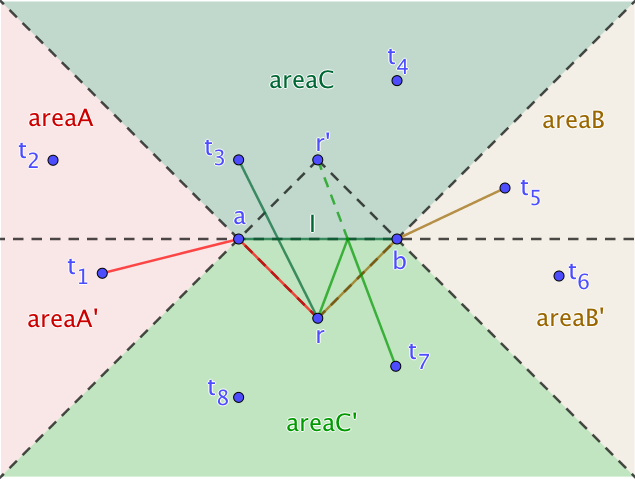
\includegraphics[width=.7\linewidth]{pic/heuristic.png}
  \caption{
    \small  
    \textbf{(i)} In $areaA \cup areaA'$, $t_1$ is the nearest to $a$;
    \textbf{(ii)} in $areaB \cup areaB'$, $t_5$ is the nearest to $b$;
    \textbf{(iii)} in $areaC$, $t_3$ is the nearest to $r$;
    \textbf{(iv)} in $areaC'$, $t_7$ is the nearest to $r'$; 
  }
  \label{fa}
\end{figure*}
\begin{itemize}
  \item Suppose the next nearest target $t$ is in $areaA \cup areaA'$ (equiv. $areaB \cup areaB'$).
    Then the optimal path must pass through the point $a$ (equiv. $b$) so the minimum $h$-value can be computed as:
    $\mathbf{min}\{d_e(r, a) + d_e(t, a)\}$ such that $t$ in $areaA \cup areaA'$
    (equiv. $areaB \cup areaB'$).
  \item Alternatively, suppose the next nearest target $t$ is instead in $areaC$.
    Then the optimal path must pass through a point $p$ in the open interval $(a, b)$.
    So the minimum $h$-value can be computed by minimising across all target points in $areaC$.
    A similar argument applies to a next nearest neighbour in $areaC'$ and we can apply the same strategy,
    but only after mirroring the root point $r$ through the interval.
    This operation is in contrast to the heuristic used by Polyanya in the point-to-point setting,
    which mirrors the target through the interval.
\end{itemize}
\noindent
Identifying the candidate target with minimum $h$-value in each of the four cases can be improved,
from a linear-time operation to NN query, by storing all of the
targets in a spatial data structure such as $R^*$-Tree~\cite{beckmann1990r}.
Thus we may compute a lower-bound estimate to the next nearest neighbour by minimising over
four candidates returned by the $R^*$-tree instead of evaluating all possible target points.

\subsection{Further Refinements}
We may notice that the Target Heuristic described thus far is potentially costly,
when compared to one constant time operation in $h_p$.
To mitigate this we could call $h_t$ less often. 
An observation is that a parent search node and its successor may use same closest target $t$
in their $h_t$. In this case, instead of running a new query, the successor can directly
inherit the $t$ from the parent.  We call this strategy \textit{lazy compute} and apply it throughout our experiments.
We find it reduces total running time by approximately 15\%.

\begin{lemma}\label{lazy-compute}
  Given search node $n=(I,r)$, its successor $n'=(I', r')$,
  and a target $t$ that minimises Euclidean distance to $n$ from among all possible candidates.
  Further suppose $h_p$(n, t) = $h_p$(n', t) .
  Then $t$ is also a target that minimises Euclidean distance to $n'$ among all possible candidates.
\end{lemma}

\begin{proof}
  If there is $t'$ closer to $n'$ than $t$, then $h_p(n', t') <
  h_p(n', t) = h_p(n, t)$, and because of Lemma~\ref{nodesc},
  $h_p(n, t') <= h_p(n', t')$, so,
  $t$ can't be the closest target of $n$, which is conflict with assumption. Thus, such $t'$
  doesn't exist.
  %$\square$
\end{proof}

Now, each search node has a target, and the search behavior should be broadly similar to 
the point-to-point setting.  But there is one significant difference:
when a nearest neighbor $t$ has been found, $t$ should no longer influence the search process.
Thus, we need to remove $t$ from search space and re-assign (i.e. update)
all search nodes in the queue which use $t$ as their closest target. 
To avoid exploring the entire queue we propose instead the following simple strategy: 
when such a node is dequeud from the open list, we apply $h_t$ to compute a new target
and we push the node back onto open all without generating any successors. 
We call this \textit{lazy reassign}.

\begin{lemma}\label{lazy-reassign}
  Let's call these search nodes who need reassignment \textbf{pseudo nodes}, and others
  \textbf{real nodes}. \textbf{Lazy reassign} never changes the relative order of real
  nodes in queue.
\end{lemma}

\begin{proof}
  Let $n_1, n_2$ be any pair of real nodes, and $s$ be any pseudo node.  After the reassignment,
  if $s$ become neither $n_1$ nor $n_2$, then inserting a third party search node has nothing to do with the relative order of $n_1$
  and $n_2$; otherwise, without the loss of generality, assume $s$ becomes $n_1$. If the relative
  order of them is $<n_2, s>$, then $f(n_2) <= f(s)$, and
  because of the definition~\ref{close}, we have $f(s) <= f(n_1)$, so
  relative order of $n_1, n_2$ doesn't change. Alternatively, if the relative order is $<s, n_2>$,
  then $n_1$  will be push to queue before $n_2$ pop out, so the relative order of $n_1, n_2$ doesn't
  change as well.%$\square$
\end{proof}

In Algorithm~\ref{hsearch}, we arrive at last at the final form of Polyanya OkNN. The algorithm
accepts either $h_v$ and $h_t$ as a heuristic function and has, in both cases, the same high level steps.

\begin{algorithm}[!ht]
  \input{./code/hsearch.pseudo}
  \caption{Polyanya OkNN}
  \label{hsearch}
\end{algorithm}

\section{Summary}
In this chapter, we start with two straightforward adaptions of point-to-point Polyany
and finally proposed two heuristics for the Polyanya OkNN algorithm.
For \textit{Interval Heuristic}, it supports multi-target by
removing $t$ from \textit{h-value}; for \textit{Target Heuristic}, it supports multi-target by
employing spatial index and computing closest target dynamically.
%Each heuristic has their
%suitable scenario, in following chapters, we will evaluate their performance under different
%scenarios (chapter~\ref{empirical})  and discuss some future improvements
%(chapter~\ref{conclusionfuture}). 

\chapter{Empirical Analysis}\label{empirical}
\section{Overview}\label{expoverview}
To evaluate Polyanya OkNN we consider two distinct setups and one large map with 
containing 9000 polygonal obstacles (this benchmark is described further in the next section).

In the first setup, targets are numerous and densely distributed throughout
the map. Our principal point of comparison in this case is \textit{LVG}~\cite{zhang2004spatial} which
is a state of the art method based on incremental visibility graphs. 
In the second setup, targets are few and sparsely distributed.
Our principal point of comparison in this case is \textit{brute-force Polyany}.
We motivate these decisions as follows:

\begin{itemize}[leftmargin=1cm]
\item When the map is large and targets are many (commonly the case in spatial database settings) \textit{LVG} considers only a small part of map and so its query processing can be very fast.
  \textit{Brute-force Polyany} meanwhile is infeasible to run (there are too many searches).

\item When the map is large targets are few ($<=10$) \textit{LVG} builds a visibility graph for almost entire map,
  and ends up with quadratic runtime complexity, which is unacceptable.
    Meanwhile, brute force \textit{Polyanya}, which is a very fast point-to-point pathfinding algorithm,
    can be competitive even when called repeatedly.
    This comparison is motivated by recent prior work involving kNN queries on road networks~\cite{abeywickrama2016k},
    where other fast point-to-point algorithms were shown to provide state-of-the-art performance in multi-targets scenarios,
    even when compared against dedicated kNN algorithms.
\end{itemize}

In experiments, we examine performance based on elapsed time and expanded search node.
For \textit{LVG}, we count the number of expanded node in \textit{Dijkstra}.

The navigation mesh of map is generated by \textit{Constrained Delaunay Triangulation}, which is $O(nlogn)$;
the implementation of such algorithm is in library \textit{Fade2D} \footnote{http://www.geom.at/fade2d/html},
the total time on such preprocessing is about 6s.
We implemented in C++ the LVG algorithm (more details below) as well as two versions of multi-target Polyanya:
one each for Target and Interval Heuristic.
Our code is compiled with \textit{clang-902.0.39.1} using \textit{-O3} flag,
under \textit{x86\_64-apple-darwin17.5.0} platform.
All of our source code and test data set are  publicly available \footnote{http://bitbucket.org/dharabor/pathfinding}
All experiments are performed on a 2.5 GHz Intel Core i7 machine with 16GB of RAM and running OSX 10.13.4. 


\section{Implementation of \textit{LVG}}\label{imptlvg}
As discussed \textit{LVG} is our primary competitor in experiments with dense targets.
However, since there is no publicly available implementation, we write one ourselves.
We implement the method as per the description in the original paper~\cite{zhang2004spatial}.
The only differences is in construction of the visibility graph:
\textit{LVG} uses the rotational plane-sweeping algorithm from~\cite{sharir1986shortest} which runs worst case $O(n^2logn)$ time.
In our work we opted to simplify development complexity and use a $R^*$-tree\cite{beckmann1990r} query for visibility checking.
Each such query runs in $log(n)$ time  and we perform one check for each unique pair of vertices.
Thus the total complexity to build a visibility graph is also $O(n^2logn)$.
This implementation, as with the rest of our code, is made publicly available.

The implmentation of $R^*$-tree we use is also publicly available \footnote{https://github.com/safarisoul/ResearchProjects/tree/master/2016-ICDE-RkFN},
and appears in other recently published work~\cite{wang2016efficiently}.

\section{Benchmark}\label{dataset}

\begin{figure*}[!hbt]
  \centering
  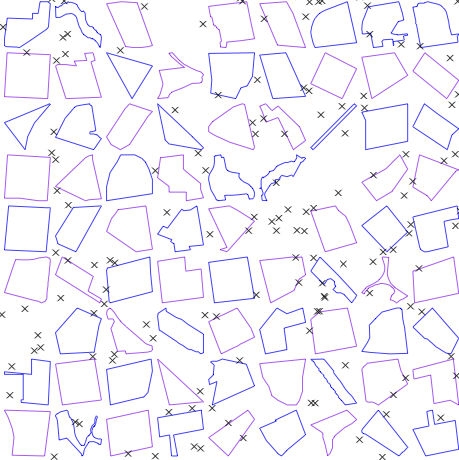
\includegraphics[width=.7\linewidth]{pic/distribution.png}
  \caption{\small Example: a generated map with many targets. Color border polygons are
  obstacles, black crosses are targets.}\label{distribution}
\end{figure*}

The data set from our main competitor LVG\cite{zhang2004spatial}
is no longer available on the public Internet so we opt to generate new benchmark problems.
We extract the shape of all parks in Australia from \textit{OpenStreetMap}\cite{OpenStreetMap} and
use these shapes as polygonal obstacles. There are about 9000 such polygons in total.
Next we generate a map by tiling all obstacles in the empty square plane.
For the tiling, we first divide the square plane into grid having $\lceil\sqrt{|O|}\rceil$ number of rows and columns.
Then we assign each polygon to a single grid cell and normalize the shape of polygon by to fit inside the cell.
Figure~\ref{distribution} gives an example a map generated in this way.
For each experiment, we're using $1000$ random query points, grouping results by
\textit{x-axis}, and computing average; the size of each bucket is at least 10. 

One thing needs to be highlighted is that,
unlike \textit{LVG} ~\cite{zhang2004spatial} where obstacles are always rectangular,
we consider polygons of arbitrary shape, which is more realistic and potentially more challenging as there are more vertices to consider.
The total number of vertices across all polygons is more than 100,000. 

\section{Experiment 1: lower bounds on performance}\label{exp1}
\begin{figure*}[!htb]
  \begin{subfigure}{\linewidth}
    \begin{subfigure}{0.5\textwidth}
        \centering
        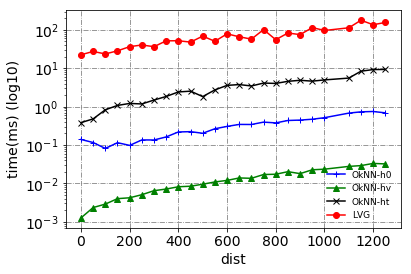
\includegraphics[width=.9\textwidth]{pic/e1_dense_time.png}
        \caption{}
        \label{e1_dense_time}
    \end{subfigure}%
    \hfill
    \begin{subfigure}{0.5\textwidth}
        \centering
        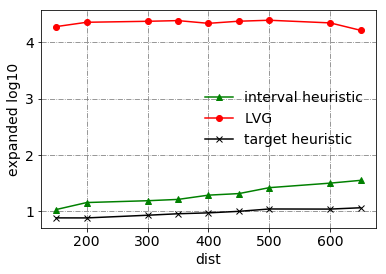
\includegraphics[width=.9\textwidth]{pic/e1_dense_gen.png}
        \caption{}
        \label{e1_dense_gen}
    \end{subfigure}
    \caption*{\small Dense experiment: $|T| \approx |O|,k=1$}
  \end{subfigure}\par\medskip
  \begin{subfigure}{\linewidth}
    \begin{subfigure}{0.5\textwidth}
        \centering
        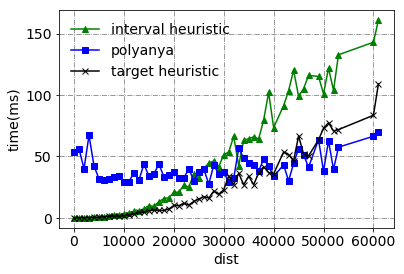
\includegraphics[width=.9\textwidth]{pic/e1_sparse_time.png}
        \caption{}
        \label{e1_sparse_time}
    \end{subfigure}%
    \hfill
    \begin{subfigure}{0.5\textwidth}
        \centering
        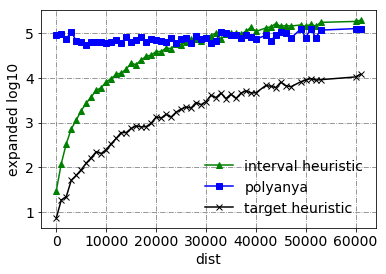
\includegraphics[width=.9\textwidth]{pic/e1_sparse_gen.png}
        \caption{}
        \label{e1_sparse_gen}
    \end{subfigure}
    \caption*{\small Sparse experiment: $|T| = 5, k=1$}
  \end{subfigure}
  \caption{\small Experiment1: examine the performance when $dist$ increase, where
  $dist$ is the obstacle distance to retrieved target}
\end{figure*}

This experiment aims to examine the performance of proposed algorithms in the easiest case, which is $k=1$.
Results show that in dense targets scenario, the proposed algorithms outperform \textit{LVG} in both space and time (fig~\ref{e1_dense_time},\ref{e1_dense_gen}).

In the sparse targets scenario, \textit{target heuristic} has the smallest number of node
operations (fig~\ref{e1_sparse_gen}), 
and both \textit{target} and \textit{interval} heuristic are outperformed on runtime by brute-force \textit{Polyanya} (fig~\ref{e1_sparse_time}) as $dist$ increases.
These results suggest the \textit{interval heuristic} has a large search space, and the
\textit{target heuristic} has a costly heuristic function. Results also show that \textit{brute-force Polyanya} is
not sensitive to $dist$, the reason is that it has to run a point-to-point search to all
targets no matter where the nearest neighbor is. 

\section{Experiment 2: computing more nearest neighbor}\label{exp2}
\begin{figure*}[!htb]
  \begin{subfigure}{\linewidth}
    \begin{subfigure}{0.5\textwidth}
        \centering
        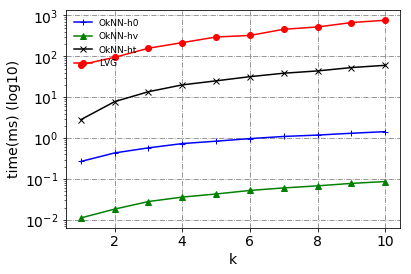
\includegraphics[width=.9\textwidth]{pic/e2_dense_time.png}
        \caption{}
        \label{e2_dense_time}
    \end{subfigure}%
    \hfill
    \begin{subfigure}{0.5\textwidth}
        \centering
        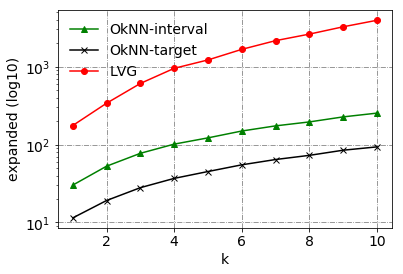
\includegraphics[width=.9\textwidth]{pic/e2_dense_gen.png}
        \caption{}
        \label{e2_dense_gen}
    \end{subfigure}
    \caption*{\small Dense: $k \in [1,...10], |T| \approx |O|$}
  \end{subfigure}\par\medskip
  \begin{subfigure}{\linewidth}
    \begin{subfigure}{0.5\textwidth}
        \centering
        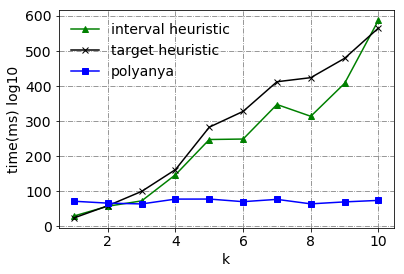
\includegraphics[width=.9\textwidth]{pic/e2_sparse_time.png}
        \caption{}
        \label{e2_sparse_time}
    \end{subfigure}%
    \hfill
    \begin{subfigure}{0.5\textwidth}
        \centering
        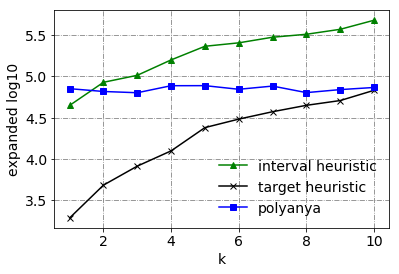
\includegraphics[width=.9\textwidth]{pic/e2_sparse_gen.png}
        \caption{}
        \label{e2_sparse_gen}
    \end{subfigure}
    \caption*{Sparse: $k \in [1,...10], |T|=10$}
  \end{subfigure}
  \caption{\small Experiment2: examine the performance when $k$ increase}
\end{figure*}
%
This experiment aims to examine the performance of algorithm when query becomes harder ($k$ increasing).
Results show that, in the dense targets scenario, the proposed algorithms still outpeform \textit{LVG}, even as $k$ increases (fig~\ref{e2_dense_time},\ref{e2_dense_gen}).
In the sparse targets scenario, results show that brute-force $Polyanya$ is not sensitive to $k$.
Meanwhile each of the two OkNN variants requires increasing amounts of node operations (and thus memory) and become quickly outperformed.
A side effect of \textit{target heuristic} when $k$ increase is that \textit{lazy reassign} causes extra node expansions.

\section{Experiment 3: changing number of targets}\label{exp3}

\begin{figure*}[!htb]
    \centering
    \begin{subfigure}{0.5\textwidth}
        \centering
        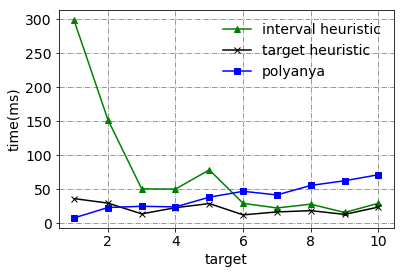
\includegraphics[width=.9\textwidth]{pic/e3_time.png}
        \caption{}
        \label{e3_time}
    \end{subfigure}%
    \hfill
    \begin{subfigure}{0.5\textwidth}
        \centering
        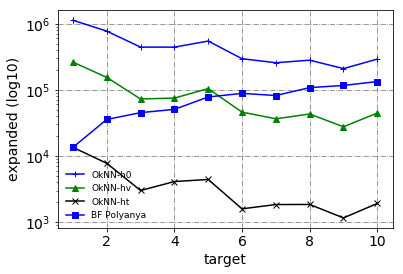
\includegraphics[width=.9\textwidth]{pic/e3_gen.png}
        \caption{}
        \label{e3_gen}
    \end{subfigure}
    \caption{\small Experiment 3: examine the performance when $|T|$ increase, $k=1, |T| \in [1,...10]$}
\end{figure*}

This experiment is run only on the sparse target set. It aims to examine the scalability of the proposed algorithms with an increasing
(but still sparse) number of targets.

Results show that proposed algorithms gradually outperform brute force \textit{Polyanya} in both time and node operations (fig~\ref{e3_time},\ref{e3_gen}).
This implies that the proposed OkNN variants algorithms are much better choices when the set of targets increase. 
Also notice that the node expansion decreases when $|T|$ goes large,
for \textit{interval heuristic}, the reason is that search nodes can reach target earlier; for
\textit{target heuristic}, in addition to previous reason, the \textit{R-tree} query in
heuristic function has good scalability. 
Although we have seen in other experiements that brute-force \textit{Polyanya} has an advantage when $k$ is large, this advantaged disappears as $|T|$ grows.
In some practical settings $|T|$ can be in the hundreds or thousands, e.g.~\cite{abeywickrama2016k} while $k$ is usually orders of magnitude smaller. 

\section{Experiment 4: behavior of target heuristic}\label{exp4}
From previous experiments, we notice that the \textit{target heuristic} always has smaller search space,
but it's sometimes orders of magnitudes slower than other competitors.
Thus, we want to dig out more details about the behavior of $h_t$.
This experiment aims to examine the target heuristic from following aspects:
\begin{itemize}
  \item the ratio of the cost on the heuristic function in total elapsed time;
  \item the ratio of the reassignment in total expanded nodes;
  \item the ratio of the heuristic function call in total expanded nodes;
\end{itemize}.

\subsection{Ratio of heuristic cost}
Figure~\ref{hcost} shows the distribution of ratio:
$\textit{heuristic cost} / \textit{total cost}$.
\begin{figure}[htp]
  \centering
  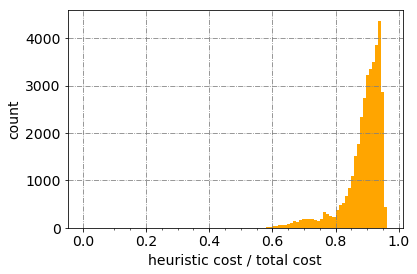
\includegraphics[width=.7\linewidth]{./pic/hcost.png}
  \caption{\small Records from experiments 1,2,3 produce the plot}
  \label{hcost}
\end{figure}
The result shows that the $h_t$ cost $\approx 90\%$ of total time, meaning that
\textit{target heuristic} needs at least an order of magnitude smaller search space 
to outperform competitors.

\subsection{Side effect}
Figure~\ref{lazy_reassign} shows the ratio of \textit{lazy reassignment} when $k$ increase.
\begin{figure}[htp]
  \centering
  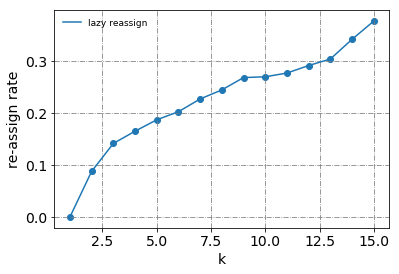
\includegraphics[width=.7\linewidth]{./pic/lazy_reassign.png}
  \caption{\small Records from experiments 1,2,3 produce the plot.}
  \label{lazy_reassign}
\end{figure}
The result shows that the side effect-\textit{reassignment} happens more freqently when $k$
increase, meaning that \textit{target heuristic} is more suitable for small $k$.

\subsection{Ratio of heuristic call}
Figure~\ref{lazy_compute} shows the distribution of ratio:
$\textit{heuristic call} / \textit{expanded nodes}$.
\begin{figure}[htp]
  \centering
  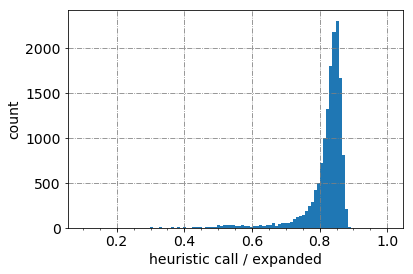
\includegraphics[width=.7\linewidth]{./pic/lazy_compute.png}
  \caption{\small Records from experiments 1,2,3 where $k=1$ produce the plot.}
  \label{lazy_compute}
\end{figure}
To ignore the side effect when $k>1$, this plot only considers those records with $k=1$.
The plot implies the effect of \textit{lazy compute} can reduce $\approx 15\%$ heuristic call in
the search.

\section{Summary}
This chapter is to evaluate proposed algorithms.
In the chapter, we've discussed the motivation of experiment design,
the benchmark problem, and results of the experiment.
From these experiements, we can see that proposed algorithms outpeform the state-of-the-art
orders of magnitudes, and between these proposed algorithms, they have different suitable
scenarios.

\chapter{Conclusion and Future Work}\label{conclusionfuture}
\section{Research Contributions}\label{contribution}

In this work we consider efficient algorithms for OkNN:
the problem of finding $k$ nearest neighbours in a plane and in the presence of obstacles.
We describe three new OkNN algorithms, all based on Polyanya~\cite{cuicompromise},
a recent and very fast algorithm for computing Euclidean-optimal shortest paths in the plane.
The first variant involves brute force search (one query per target point).
The second and third variants involves running Polyanya as a multi-target algorithm but with added heuristic guidance.
We develop two new online and admissible heuristics for this purpose: the Interval Heuristic and the Target Heuristic.

We compare these variant algorithms against one another and against LVG~\cite{zhang2004spatial},
an influential and state of the art OkNN method based on incremental visibility graphs.
The headline result from our experiment is that Polyanya OkNN can be up to
\textbf{three orders of magnitude} faster than LVG.

Moreover, each of the three variants appears best suited to particular OkNN settings:
\textbf{brute-force Polyanya} is highly effective when the number of candidates is small (independent of $k$);
the \textbf{Interval Heuristic} works well when targets are many (again, independent of $k$);
the \textbf{Target Heuristic} works well when targets are few and $k$ is also small.

The work has been accepted for publication on \textit{Proceedings of the 11th Annual Symposium on Combinatorial Search (SoCS’2018), colocated with
IJCAI/ECAI’2018, July 2018}.

\section{Future Works}\label{future}
We also consider future works in following directions.
Firstly, due to the high performance of proposed algorithms, we believe they can be used to
speed up other types of spatial query which need to compute obstacle distance,
as described in section~\ref{lrquery}.

Secondly, we can improve heuristic function in \textit{target heuristic}.
In experiments, we notice that the \textit{target heuristic} cost $\approx 80\%$ of
total running time on NN query, and one possible way is combining four queries into one.
Besides, in literature review, we mainly focus on \textit{R-tree} and its variants which
have good scalability on dimensions, however, in our case, the dimension is always two (maybe
three in 3D extension). Thus, other high performance low-dimension data structures may helpful,
e.g. \textit{KD-tree}\cite{ooi1987spatial} and
\textit{Locality-sensitive hashing}\cite{slaney2008locality}.

Thirdly, \textit{brute-force Polyanya} can be improved by smart pruning. We notice that
the \textit{brute-force Polyanya} outperforms other proposed algorithms in sparse scenario,
thus, instead of considering all targets,
a pruning strategy like \textit{fast filter}\cite{xia2004fast} may make it work in general
scenario.


\pagebreak
\bibliographystyle{plain}
\bibliography{refs}
\appendix
\chapter{Dataset}
\begin{figure}[htb]
  \centering
  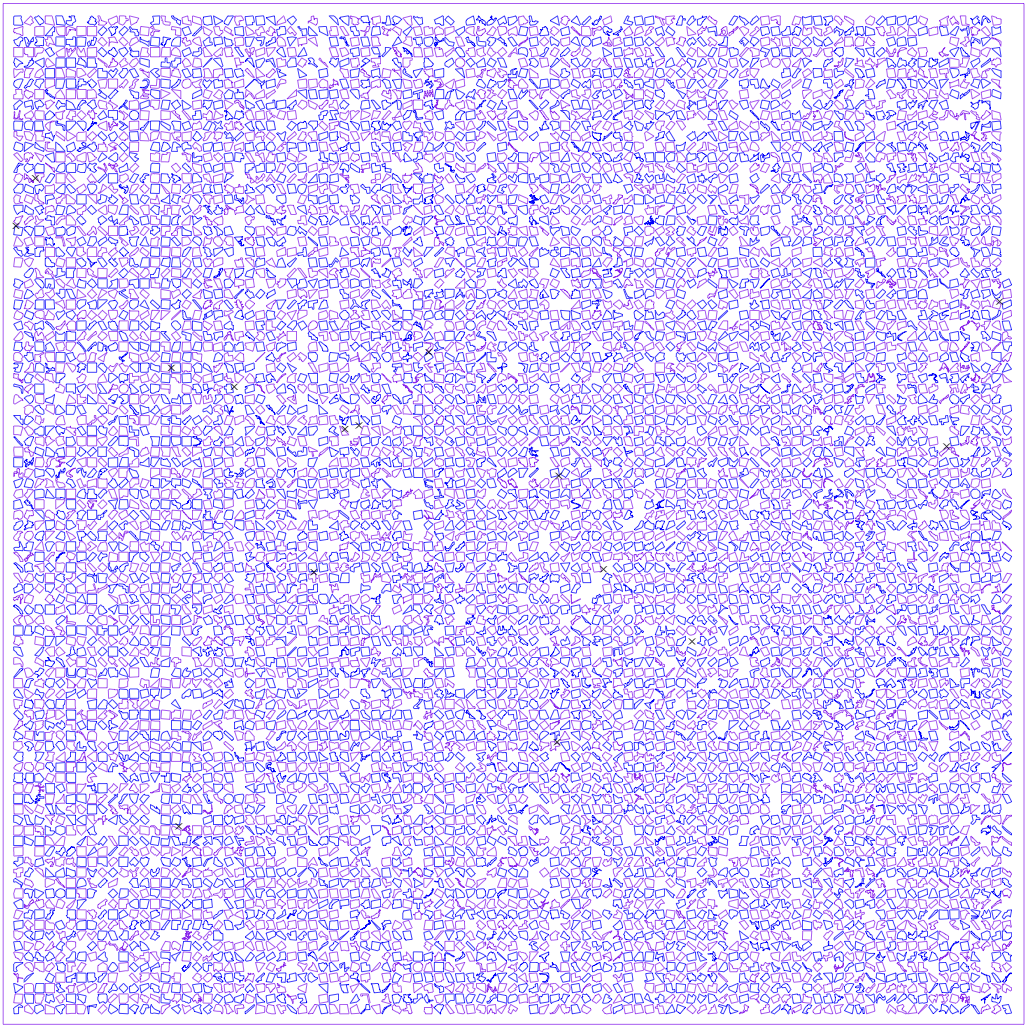
\includegraphics[width=\linewidth]{./pic/poly9000.png}
  \caption{\small The map in experiments, it has nearly 9000 polygonal obstacles, and 10,000
  vertexes.}
\end{figure}
\chapter{Source Code}
\lstinputlisting[caption=extract shape of parks, label=park2poly]{./code/park2poly.h}
\newpage
\lstinputlisting[caption=generate targets, label=gentarget]{./code/genPoints.h}
\newpage
\lstinputlisting[caption=target heuristic, label=heuristic_function]{./code/heuristic}
\newpage
\lstinputlisting[caption=final OkNN, label=oknn]{./code/knnheuristic.cpp}
\newpage

\end{document}
